\documentclass[usenames,a4,portrait,semhelv]{seminar}

\usepackage{pst-all}
\usepackage{pst-blur}
\usepackage{amsmath}
\usepackage[dvips,pdftex]{graphicx}
\usepackage[activeacute,spanish]{babel}
\usepackage{amsbsy}
%\usepackage{amssymb}
\usepackage{pifont}
\usepackage[latin1]{inputenc}
%\usepackage[nocfg]{pdfslide}
\usepackage{pause}
\usepackage{url}
\usepackage{fvrb-ex}
\usepackage{zahlen}
\usepackage{semcolor}
\usepackage{semlayer}
\input{seminar.bug}
\input{seminar.bg2}

%\usepackage{pifont}
\usepackage{marvosym}

%\usepackage[dvips]{graphicx}

%%%%%%%%%%%%%%%%%%%%%%%%%%%%%%%%%%%%%%%%%%%%%%%%%%%%%%%%%%%%%%%%%%%%%%%%%%
%%% directory from where eps-files are included
%%% list of directories like {{dir1}{dir2}...}

\graphicspath{{./}}

%%%%%%%%%%%%%%%%%%%%%%%%%%%%%%%%%%%%%%%%%%%%%%%%%%%%%%%%%%%%%%%%%%%%%%%%%%
%%% set some parameters

\def\initials{AO}
\def\name{Antalcides Olivo}
\def\place{Repaso de Estad�stica} % `place' or 'conference, place'
\def\month{07/2003} % format 'MM/YYYY'

%%%%%%%%%%%%%%%%%%%%%%%%%%%%%%%%%%%%%%%%%%%%%%%%%%%%%%%%%%%%%%%%%%%%%%%%%%
%%% page-style

\renewcommand{\slidetopmargin}{.4in}
\addtolength{\slidewidth}{1in}
\extraslideheight{10mm}

\newcommand{\footcolor}{\Black}
\newcommand{\headtext}{}

\newsavebox{\myLoewe}
\sbox{\myLoewe}{
\includegraphics[scale=0.5]{logofoto.eps}}

\newpagestyle{mystyle}
{%
\rput[l]{0}(0,0)%
   {\psframebox[fillstyle=gradient,
                linecolor=White,
                gradmidpoint=0.45,
                gradlines=100,
                gradangle=90]
                {\begin{minipage}{0.98\textwidth}
                 {\large\bf \initials}
                 \quad
                 \rput{0}(0.2,0.11){\usebox{\myLoewe}}
                 \qquad\qquad
                 {\bf \place - \month}
                 \hfill\hfill\Red{\large\bf \headtext}
                 \end{minipage}}}
}% end header box
{%
\begin{minipage}{\textwidth}
\vspace*{-4truemm}
\hrulefill\\
\phantom{.}\hfill \footcolor{\name, \month}\hfill --\thepage--
\end{minipage}
}% end footer box

\slideframe{none}
\pagestyle{mystyle}


%%%%%%%%%%%%%%%%%%%%%%%%%%%%%%%%%%%%%%%%%%%%%%%%%%%%%%%%%%%%%%%%%%%%%%%%%%
%%% color-stuff

\definecolor{LightGray}{rgb}{0.94,0.94,0.94}
\definecolor{VeryLightBlue}{rgb}{0.9,0.9,1}
\definecolor{LightBlue}{rgb}{0.8,0.8,1}
\definecolor{DarkBlue}{rgb}{0,0,0.6}
\definecolor{LightGreen}{rgb}{0.88,1,0.88}
\definecolor{MidGreen}{rgb}{0.6,1,0.6}
\definecolor{DarkGreen}{rgb}{0,0.6,0}
\definecolor{VeryLightYellow}{rgb}{1,1,0.9}
\definecolor{LightYellow}{rgb}{1,1,0.6}
\definecolor{MidYellow}{rgb}{1,1,0.5}
\definecolor{VeryLightRed}{rgb}{1,0.9,0.9}
\definecolor{LightRed}{rgb}{1,0.8,0.8}

\newcommand{\VeryLightBlue}[1]{{\color{VeryLightBlue}{#1}}}
\newcommand{\LightBlue}[1]{{\color{LightBlue}{#1}}}
\newcommand{\Blue}[1]{{\color{Blue}{#1}}}
\newcommand{\DarkBlue}[1]{{\color{DarkBlue}{#1}}}
\newcommand{\DarkGreen}[1]{{\color{DarkGreen}{#1}}}
\newcommand{\VeryLightRed}[1]{{\color{VeryLightRed}{#1}}}
\newcommand{\LightRed}[1]{{\color{LightRed}{#1}}}
\newcommand{\Red}[1]{{\color{Red}{#1}}}
\newcommand{\Gray}[1]{{\color{Gray}{#1}}}
\newcommand{\Black}[1]{{\color{Black}{#1}}}

%%%%%%%%%%%%%%%%%%%%%%%%%%%%%%%%%%%%%%%%%%%%%%%%%%%%%%%%%%%%%%%%%%%%%%%%%%
%%% newcommands

\newcommand{\fnz}{\footnotesize}

%%%%%%%%%%%%%%%%%%%%%%%%%%%%%%%%%%%%%%%%%%%%%%%%%%%%%%%%%%%%%%%%%%%%%%%%%%
\begin{document}

% switch-on cumulative overlays
\makeatletter
\def\pst@initoverlay#1{%
\pst@Verb{%
/BeginOL {dup (all) eq exch TheOL le or {IfVisible not {Visible
/IfVisible true def} if} {IfVisible {Invisible /IfVisible false def} if}
ifelse} def
\tx@InitOL /TheOL (#1) def}}
\makeatother

% set some style parameters
\renewcommand{\headtext}{title}
\psset{gradbegin=MidYellow,gradend=MidGreen}
\renewcommand{\footcolor}{\DarkGreen}

%%%%%%%%%%%%% slide 1 %%%%%%%%%%%%%
\begin{slide}
\begin{center}

\psblurbox[fillstyle=solid,fillcolor=yellow,linecolor=red]
{\Blue{\huge\bf �Qu� es la estad�stica?}}
%% This document created by Scientific Word (R) Version 3.5

%TCIDATA{LaTeXparent=0,0,Est12.tex}
%TCIDATA{ChildDefaults=%
%chapter:2,page:33
%}


%\chapter{Medidas descriptivas}

\subsection{Medidas de tendencia central}

\subsection{Medias}

\subsubsection{Media aritm\'{e}tica}

La media aritm\'{e}tica de una muestra \ es la suma de cada uno de los valores
posibles multiplicado por su frecuencia, es decir.

Si la siguiente tabla \ representa la tabla de frecuencia de la muestra%

\[%
\begin{tabular}
[c]{|l|l|l|}\hline
$M$ & $n_{i}$ & $f_{i}$\\\hline
$x_{1}$ & $n_{1}$ & $f_{1}$\\\hline
$\vdots$ & $\vdots$ & $\vdots$\\\hline
$x_{k}$ & $n_{k}$ & $f_{k}$\\\hline
\end{tabular}
\]

La media es el valor :
\begin{equation}
\overset{\_}{x}=\frac{\overset{k}{\sum_{i=1}}x_{i}n_{i}}{n} \label{2-1}%
\end{equation}
y si los datos no est\'{a}n ordenados entonces $\ $%
\begin{equation}
\overset{\_}{x}=\frac{\overset{k}{\sum_{i=1}}x_{i}}{n} \label{2-2}%
\end{equation}%

\begin{remark}
En la definici\'{o}n de media se consider\'{o} que la variable de inter\'{e}s
$X$ es discreta, pero si la variable $X$ no es discreta sino continua. En la
f\'{o}rmula se reemplaza cada valor $x_{i}$ por la marca de clase
correspondiente es decir
\begin{equation}
\overset{\_}{x\,}=\frac{\overset{k}{\sum_i=1}m_in_i}{n} \label{2-3}
\end{equation}
\end{remark}

Este proceso hace que la media aritm\'{e}tica difiera de la media obtenida
seg\'{u}n (2.1), es decir habr\'{a} una perdida de precisi\'{o}n que ser\'{a}
mayor en cuanto mayor sea la diferencia entre las marcas de clase y los
valores reales, o sea entre mayor sea la longitud $a_{i}$ de los intervalos\ \ \ \ \ \ \ \ \ \ \ \ \ \ \ \ \

\subparagraph{Desventajas de la media}

La media es una medida muy usa\-da en estad\'{\i}stica, pero a pesar de eso
posee ciertas desventajas

\begin{itemize}
\item La media aritm\'{e}tica es muy sensible a los valores extremos, es decir
si una medida se aleja mucho de las otras har\'{a} que la media se aproxime
mucho a ella

\item No se recomienda usar cuando los datos se desplazan hacia los extremos

\item En el caso de variables continuas depende de los intervalos de clase

\item en le caso de variables discretas el valor puede no ser un valor de la muestra.
\end{itemize}

\subsubsection{}

Otra media es la llamada media cuadr\'{a}tica $\overset{\_}{x}_{c}$la cual es
la ra\'{\i}z cuadrada de la media aritm\'{e}tica de los cuadrados
\[
\overset{\_}{x}_{c}=\sqrt{\frac{\sum_{i=1}^{n}x_{i}^{2}}{n}}%
\]

\subsection{La mediana}

Sea $X$ una variable discreta cuyas observaciones han sido ordenadas de mayor
de mayor a menor, entonces se le llama mediana $\widetilde{x}$ al primer valor
de la variable que deja por debajo de si el 50\% de las observaciones es decir
si $n$ es el n\'{u}mero de observaciones, la mediana ser\'{a} la
observaci\'{o}n $\left[  |\frac{n}{2}|\right]  +1$%

\begin{definition}
Sea $x_{(1),}x_{(2)},x_{(3)},\cdots,x_{(n)}$ las observaciones de una muestra
para una variable $X$ donde $x_{(1)}$ representa la observaci\'{o}n m\'{a}s
peque\~{n}a, $x_{(2)}$ la observaci\'{o}n que le sigue en valor y as\'{\i}
sucesivamente $x_{(n)}$ denota la observaci\'{o}n de mayor valor, entonces la
mediana se define \[ \widetilde{x}=\left\{
\begin{tabular}
[c]{ll}
$x_{([n+1]/2)}$ & si $n$ impar\\ $\frac{x_{(n/2)}+x_{([n/2]+1)}}{2}$ & si $n$
par
\end{tabular}
\right.  \]
\end{definition}

En el caso de variables continuas, las clases vienen dadas por intervalos como
se indic\'{o} en el cap\'{\i}tulo anterior por tal raz\'{o}n para determinar
la mediana se escoge el intervalo donde se encuentra el valor para el cual
est\'{a}n debajo de \'{e}l la mitad de los datos. Entonces a partir de ese
intervalo se observan las frecuencias absolutas acumuladas y se aplica la
siguiente f\'{o}rmula
\[
\widetilde{x}=x_{i-1}+\frac{\frac{n}{2}-N_{i-1}}{n_{i}}a_{i}%
\]
de aqu\'{\i} se puede deducir que $\widetilde{x}$ el ``punto'' que divide al
histograma en dos partes de \'{a}reas iguales

\subsubsection{Propiedades y desventajas de la mediana}

\begin{enumerate}
\item Tiene la ventaja de no ser afectada por los valores extremos y por eso
se aconseja para distribuciones para las cuales los datos no se concentran en
el centro

\item Es f\'{a}cil de calcular

\item En el caso de variables discretas el valor de la mediana es un valor de
la variable

\item El mayor defecto es que las propiedades matem\'{a}ticas son muy
complicadas y esto hace que muy poco se use para realizar inferencias

\item Es funci\'{o}n de los intervalos escogidos en el caso de variables continuas
\end{enumerate}

\subsubsection{La moda}

Llamaremos moda $\widehat{x}$ a cualquier m\'{a}ximo relativo de la
distribuci\'{o}n de frecuencias, es decir, cualquier valor de la variable que
posea una frecuencia mayor que su anterior y posterior valor.

En el caso de variables continuas es m\'{a}s correcto hablar de intervalos
modales. Luego de determinar el intervalo de clase o intervalo modal,que es
aquel para el cual la distribuci\'{o}n de frecuencia posee un m\'{a}ximo
relativo, se determina la moda utilizando la siguiente f\'{o}rmula
\[
\widehat{x}=x_{i-1}+\frac{n_{i}-n_{i-1}}{\left(  n_{i}-n_{i-1}\right)
+\left(  n_{i}-n_{i+1}\right)  }a_{i}%
\]

\paragraph{Propiedades de la moda\newline }

La moda posee la siguientes propiedades

\begin{itemize}
\item Es muy f\'{a}cil de calcular

\item Puede no ser \'{u}nica

\item Es funci\'{o}n de los intervalos de su amplitud,n\'{u}mero y l\'{\i}mites
\end{itemize}

\subsubsection{Relaci\'{o}n entre la media, la moda y la mediana}

En el caso de distribuciones unimodales, la mediana est\'{a} con frecuencia
comprendida entre la media y la moda (incluso m\'{a}s cerca de la media).

En distribuciones que presentan cierta inclinaci\'{o}n, es m\'{a}s aconsejable
el uso de la mediana. Sin embargo en estudios relacionados con prop\'{o}sitos
estad\'{\i}sticos y de inferencia suele ser m\'{a}s apta la media.

Veamos un ejemplo de c\'{a}lculo de estas tres magnitudes.

\section{Medidas de posici\'{o}n}

A veces es importante obtener los valores de la variable que divi\-den la
poblaci\'{o}n en cuatro,diez o cien partes iguales,usualmente llamados
cuartiles deciles y percentiles respectivamente.

El procedimiento es similar al utilizado para determinar la mediana, como lo
indicaremos ahora.

\subsubsection{Percentil}

Para una variable discreta, se define el percentil de orden $k,$ como la
observaci\'{o}n que deja por debajo de si el $k\%$ de la poblaci\'{o}n es
decir
\begin{align*}
N_{k}  &  =n\frac{k}{100},\text{ si }n\text{ es impar}\\
\text{es decir }p_{k}  &  =x_{[|(n+1)\frac{k}{100}|]}%
\end{align*}
donde en sub \'{\i}ndice $[|(n+1)\frac{k}{100}|]$ indica que es la
posici\'{o}n $k$ a la que le corresponde ese valor de la frecuencia absoluta
acumulada. Si $n$ es par
\[
p_{k}=\frac{x_{[|n\frac{k}{100}|]}+x_{[|n\frac{k}{100}|]+1}}{2}%
\]

En el caso de variables continuas se busca el intervalo donde se encuentra
\ $p_{k},$ es decir se busca el valor que deja por debajo de si el $k\%$ de
las observaciones y se determina el intervalo $(x_{i-1,}x_{i}]$ donde se
encuentra y se utiliza la relaci\'{o}n
\[
p_{k}=x_{i-1}+\frac{n\frac{k}{100}-N_{i-1}}{n_{i}}\cdot a_{i}%
\]

\subsubsection{Quartiles}

Los cuartiles son tres y se definen:

\begin{itemize}
\item $Q_{1}=p_{25}$

\item $Q_{2}=p_{50}$

\item $Q_{3}=p_{75}$
\end{itemize}

\subsection{Deciles}

De manera an\'{a}loga se definen los deciles

los deciles son los valores que dividen las observaciones en 10 grupos de
igual tama\~{n}o es decir son el conjunto

$D_{1},D_{2},D_{3},\cdots,D_{10}$ y se definen

$D_{i}=p_{10\cdot i}\qquad i=1,2,3,\cdots,10$

\section{Medidas de variabilidad o dispersi\'{o}n}

\subsection{Varianza y desviaci\'{o}n t\'{\i}pica}

Como forma de medir la dispersi\'{o}n de los datos hemos descartado:

La varianza, $S_{n}^{2}$, se define como la media de las diferencias
cuadr\'{a}ticas de $n$ puntuaciones con respecto a su media aritm\'{e}tica, es
decir
\[
S_{n}^{2}=\frac{1}{n}\sum_{i=1}^{n}\left(  x_{i}-\overline{x}\right)  ^{2}%
\]

Para datos agrupados en tablas, usando las notaciones establecidas en el
cap\'{\i}tulo anterior, la varianza se puede escribir como
\[
S_{n}^{2}=\frac{1}{n}\sum_{i=1}^{k}\left(  x_{i}-\overline{x}\right)
^{2}\cdot n_{i}%
\]

Una f\'{o}rmula equivalente para el c\'{a}lculo de la varianza est\'{a} basada
en lo siguiente:
\[
S_{n}^{2}=\frac{1}{n}\sum_{i=1}^{n}x_{i}^{2}n_{i}-\overline{x}^{2}%
\]

La varianza no tiene la misma magnitud que las observaciones (ej. si las
observaciones se miden en metros, la varianza lo hace en $metros^{2}$ ). Si
queremos que la medida de dispersi\'{o}n sea de la misma dimensionalidad que
las observaciones bastar\'{a} con tomar su ra\'{\i}z cuadrada. Por ello se
define la desviaci\'{o}n t\'{\i}pica, $S_{n}$, como
\[
S_{n}=\sqrt{S_{n}^{2}}%
\]

\overlay{2}{%
\DarkGreen{\item
\Black{
%% This document created by Scientific Word (R) Version 3.5

\documentclass{article}%
\usepackage{amsmath}%
\usepackage{amsfonts}%
\usepackage{amssymb}%
\usepackage{graphicx}
%TCIDATA{OutputFilter=latex2.dll}
%TCIDATA{LastRevised=Tuesday, July 22, 2003 14:31:06}
%TCIDATA{<META NAME="GraphicsSave" CONTENT="32">}
\section{Teor\'{\i}a de probabilidades}
\section{Experimentos y sucesos aleatorios}
\begin{definition}
Diremos que un experimento es aleatorio si se veri\-fican las siguientes condiciones,
\begin{enumerate}
\item Se puede repetir indefinidamente, siempre con las mismas condiciones.
\item Antes de realizarlo no se puede predecir el resultado.
\item El resultado ''$e"$ que se obtiene pertenece a un conjunto de resultados
posibles conocido previamente el cual llamaremos espacio muestral y lo
denotaremos con la letra $\Omega\;o\;S$. Los elementos del espacio muestral se
denominan sucesos elementales.
\end{enumerate}
\end{definition}
Es decir si $e_{1},e_{2}\in S\Longrightarrow e_{1},e_{2}$ son sucesos
elementales o puntos muestrales.En otras palabras: Un suceso es elemental si
su ocu\-rrencia o no ocurrencia no est\'{a} relacionada con ning\'{u}n otro suceso.
Cualquier subconjunto $A$ de $S$ se denomina suceso o evento aleatorio.
El espacio muestral puede ser de dos tipos:
\begin{itemize}
\item Discreto si est\'{a} formado por un conjunto finito o numerable de resultados.
\item Continuo si est\'{a} compuesto por un conjunto no numerable de elementos.
\end{itemize}
\begin{definition}
[Suceso determinista]Se denomina experimento determinista a el experimento que
al realizarlo varias veces con las mismas condiciones iniciales obtenemos
siempre el mismo resultado
\end{definition}
\begin{example}
Si dejamos caer dos cuerpos de diferentes masas y a la misma altura en el
vac\'{\i}o, los dos cuerpos caer\'{a}n al mismo tiempo.
\end{example}
Cuando en un experimento no se puede predecir el resultado final, decimos que
el experimento es aleatorio
\begin{example}
En una ruleta legal no se sabe que n\'{u}mero va a salir
\end{example}
\subsection{Probabilidad de laplace}
Si un experimento cualquiera se puede repetir obteniendo un n\'{u}mero finito
de resultados posibles y no existe ninguna raz\'{o}n para pensar que un
resultado tiene privilegios sobre otro, se calcula la probabi\-lidad del
suceso $A$ seg\'{u}n la regla de Laplace
\[
P\left(  A\right)  =\frac{n\acute{u}mero\,de\,casos\,favorables\,para\,A}{n\acute{u}mero\,de\,casos\,posibles}=\frac{n\left(  A\right)  }{n\left(
S\right)  }
\]
\begin{example}
Calcular la probabilidad de que al lanzar un dado se obtenga un n\'{u}mero par
\end{example}
\begin{solution}
El espacio muestral es $S=\{1,2,3,4,5,6\}$ llamaremos $A$ al suceso que da
como resultado un n\'{u}mero par el lanzamiento del dado, $A=\{2,4,6\},$ si
suponemos que el dado es legal, es decir ninguna cara tiene privilegio sobre
otra para salir, entonces
\[
P\left(  A\right)  =\frac{n\left(  A\right)  }{n\left(  S\right)  }=\frac
{3}{6}=\frac{1}{2}
\]
\end{solution}
\begin{definition}
\textbf{Definici\'{o}n axiom\'{a}tica de probabilidad}\newline Dado un espacio
muestral $S$, y una $\sigma-\acute{a}lgebra$ de sucesos $\mathcal{A}$ sobre
\'{e}l, diremos que $P$ es una probabilidad sobre $\mathcal{A}$ si cumple las
siguientes propiedades
\begin{description}
\item[A$_{1}$] La probabilidad es una funci\'{o}n definida sobre
$\ \mathcal{A}$, que toma solo valores positivos comprendidos entre 0 y 1, es
decir
\[
\begin{array}
[c]{ccc}
P:\mathcal{A} & \rightarrow & [0,1]\subset IR\\
A\in\mathcal{A} & \mapsto & 1\geq P\left(  A\right)  \geq0
\end{array}
\]
\item[A$_{2}$] La probabilidad del suceso seguro es 1
\[
P\left(  S\right)  =1
\]
\item[A$_{3}$] Para cualquier sucesi\'{o}n infinita $A_{1},A_{2},A_{3},\cdots$
de sucesos disjuntos de $\mathcal{A}$ se tiene que la probabilidad de el
evento $\bigcup_{i=1}^{\infty}A_{i}$ es la serie infinita de las
probabilidades, es decir
\end{description}
\end{definition}
\[
P\left(  \bigcup_{i=1}^{\infty}A_{i}\right)  =\sum_{i=1}^{\infty}P\left(
A_{i}\right)
\]
\subsubsection{propiedades}
$P\left(  \phi\right)  =0$
\begin{theorem}
Para cualquier sucesi\'{o}n finita de $n$ eventos disjuntos $A_{1},A_{2}
,A_{3},\cdots A_{n}\in\mathcal{A}$
\[
P\left(  \bigcup_{i=1}^{n}A_{i}\right)  =\sum_{i=1}^{n}P\left(  A_{i}\right)
\]
\end{theorem}
\begin{theorem}
para cualquier suceso $A\in\mathcal{A}$ se tiene que $P\left(  A^{\prime
}\right)  =1-P\left(  A\right)  $
\end{theorem}
\begin{theorem}
Si $A,B\in\mathcal{A}$ y $A\subset B$, entonces $P\left(  B\right)  \geq
P\left(  A\right)  $ y del A$_{1}$ $P\left(  B\cap A^{\prime}\right)  \geq0$
de lo que se deduce $P\left(  B\right)  \geq P\left(  A\right)  $
\end{theorem}
\begin{center}
\end{center}
\begin{theorem}
Para dos sucesos $A,B\subset\mathcal{A}$ cualesquiera $P\left(  A\cup
B\right)  =P\left(  A\right)  +P\left(  B\right)  -P\left(  A\cap B\right)  $
\end{theorem}
\begin{example}
Un estudiante de clase puede ser hombre o mujer. Si la probabilidad de que un
hombre sea seleccionado es 0.3 \textquestiondown Cu\'{a}l es la probabilidad
de que sea seleccionada una mujer?
\begin{solution}
Sea $A$ el evento de que se seleccione un hombre de la clase y sea $B$ el
evento de seleccionar una mujer, entonces es obvio que $S=A\cup B,$ y
adem\'{a}s $A\cap B=\phi,$ aplicando el teorema 7
\[
P\left(  A\cup B\right)  =P\left(  A\right)  +P\left(  B\right)  -P\left(
A\cap B\right)
\]
y de los teorema 4 y A$_{2}$ obtenemos
\begin{align*}
1  &  =P\left(  A\right)  +P\left(  B\right) \\
1  &  =0,3+P\left(  B\right) \\
P\left(  B\right)   &  =0,7
\end{align*}
\end{solution}
\end{example}
\begin{example}
Se selecciona una bola de una urna que contiene bolas rojas, blancas, azules,
amarillas y verdes. Si la probabilidad de seleccionar una bola roja es
$\frac{1}{5}$ y la de seleccionar una blanca es $\frac{2}{5}$
\textquestiondown Cu\'{a}l es la probabilidad de seleccionar una bola azul,
amarilla o blanca?
\end{example}
\begin{solution}
Sean $A_{1},A_{2},A_{3},A_{4},A_{5},A_{6}$ los eventos de seleccionar de la
urna una bola roja, blanca, azul, amarilla y verde respectivamente. Nos dicen
que $P\left(  A_{1}\right)  =$ $\frac{1}{5}$ y $P\left(  A_{2}\right)
=\frac{2}{5}$, entonces
\[
P\left(  A_{3}\cup A_{4}\cup A_{5}\cup A_{6}\right)  =P\left(  B\right)  =?
\]
Como los eventos son disjuntos
\[
S=A_{1}\cup A_{2}\cup A_{3}\cup A_{4}\cup A_{5}\cup A_{6}
\]
y por A$_{2}$ y el th.3
\begin{align*}
1  &  =P\left(  A_{1}\right)  +P\left(  A_{2}\right)  +P\left(  B\right) \\
P\left(  B\right)   &  =1-\frac{1}{5}-\frac{2}{5}=\frac{2}{5}
\end{align*}
\end{solution}
\begin{example}
Si la probabilidad de que un estudiante A pierda un examen de estad\'{\i}stica
es de 0,5, la probabilidad de que un estudiante B pierda el mismo examen es de
0,2 y la probabilidad de que ambos pierdan el examen es de 0,1
\end{example}
\begin{enumerate}
\item \textit{\textquestiondown Cu\'{a}l es la probabilidad de que al menos
uno de estos estudiantes gane el examen?}
\item \textit{\textquestiondown Cu\'{a}l es la probabilidad de de que ninguno
de los dos pierda el examen?}
\end{enumerate}
\begin{solution}
Sea $A$ el evento que el estudiante A pierda el examen y sea $B$ el evento de
que el estudiante B pierda el examen de estad\'{\i}stica
\end{solution}
\begin{description}
\item \textit{Nos piden la probabilidad de que uno de los dos gane el examen
pero no los dos, es decir si }$C$ \textit{es} \textit{este evento}
\begin{align*}
P\left(  C\right)   &  =P\left(  A^{\prime}\right)  +P\left(  B^{\prime
}\right)  -P\left(  A^{\prime}\cap B^{\prime}\right) \\
P\left(  A^{\prime}\right)   &  =1-P\left(  A\right)  =1-0,5=0,5\\
P\left(  B^{\prime}\right)   &  =1-P\left(  B\right)  =1-0,2=0,8\\
A^{\prime}\cap B^{\prime}  &  =\left(  A\cup B\right)  ^{\prime}\\
P\left(  A^{\prime}\cap B^{\prime}\right)   &  =1-P\left(  A\cup B\right)
\end{align*}
\textit{Pero}
\begin{align*}
P\left(  A\cup B\right)   &  =P\left(  A\right)  +P\left(  B\right)  -P\left(
A\cap B\right)  =0,6\\
P\left(  A^{\prime}\cap B^{\prime}\right)   &  =0,4
\end{align*}
\textit{entonces}
\[
P\left(  C\right)  =0,5+0,8-0,4=0,9
\]
\item $P\left(  A^{\prime}\cap B^{\prime}\right)  =0,4$
\end{description}
\section{T\'{e}cnica para la enumeraci\'{o}n de puntos muestrales}
Cuando $S$ o cualquiera de sus subconjuntos tiene muchos eventos elementales
describirlo por extensi\'{o}n para determinar los casos favorables y casos
posibles se hace engorroso por lo que en esta se\-cci\'{o}n utilizaremos el
an\'{a}lisis combinatorio para determinar los casos favorables y posibles de
una manera m\'{a}s simple.
\subsection{Diagrama de \'{a}rbol}
En experimentos simples es muy \'{u}til utilizar un m\'{e}todo llamado
diagrama de \'{a}rbol el cual explicar\'{e} con un ejemplo.
\begin{example}
Si se lanza una moneda legal tres veces \textquestiondown Cu\'{a}l es la
probabilidad de que \ en la primera y la ultima lanzada salga cara?.
%BeginExpansion
\begin{figure}
[ptb]
\begin{center}
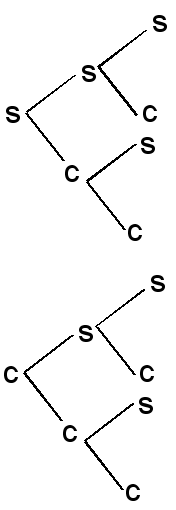
\includegraphics[
natheight=7.083700in,
natwidth=2.444800in,
height=2.7034in,
width=0.9504in
]{g11ir300.png}
\end{center}
\end{figure}
%EndExpansion
\end{example}
\begin{solution}
En el diagrama observamos que para el primer lanzamiento hay dos posibilidades
sello ($S$) y cara ($C$) en el segundo lanzamiento para cada posibilidad
anterior hay dos nuevas posibilidades y en el tercer se da lo mismo por lo que
al final hay 8 casos posibles y dos casos favorables de acuerdo con Laplace,
entonces si $A$ es el evento que sale cara en el primer y \'{u}ltimo
lanzamiento
\[
P\left(  A\right)  =\frac{2}{8}=\frac{1}{4}
\]
\end{solution}
\begin{theorem}
Consid\'{e}rese un experimento que tiene las dos cara\-cter\'{\i}sticas siguientes
\end{theorem}
\begin{itemize}
\item \textit{El experimento se realiza en dos partes }
\item \textit{La primera parte del experimento tiene }$m$ \textit{resultados
posibles }$x_{1},x_{2},x_{3},\cdots,x_{m}$ \textit{independientemente del
resultado} $x_{i}$ \textit{obtenido la segunda parte del experimento tiene
}$n$\textit{\ resultados posibles }$y_{1},y_{2},y_{3},\cdots,y_{n}
$\textit{.\newline Cada resultado del espacio muestral S del experimento
ser\'{a} por tanto, un par de la forma }$\left(  x_{i},y_{j}\right)
$\textit{\ es decir }
\begin{align*}
S  &  =\left\{  \left(  x_{i},y_{j}\right)  |i=1,2,3,\cdots m;j=1,2,3\cdots
n\right\} \\
n\left(  S\right)   &  =mn
\end{align*}
\end{itemize}
Este teorema puede generalizarse de la siguiente forma
Si un experimento \ puede realizarse con las siguientes caracter\'{\i}sticas
\begin{itemize}
\item El experimento se realiza en $k$ partes
\item la primera parte puede realizarse con $n_{1}$ resultados posibles
$x_{11},x_{12},x_{13},\cdots,x_{1n_{1}}$ e independientemente del resultado
$x_{1i}$ se pueden realizar la segunda parte con $n_{2}$ resultados posibles
$x_{21},x_{22},x_{23},\cdots,x_{2n_{2}}$ y as\'{\i} sucesivamente cada parte
del experimento puede realizarse de $n_{l}$ formas, $l=1,2,3,\cdots k$
obteni\'{e}ndose un espacio muestral de la forma
\begin{align*}
S  &  =\{(x_{1i},x_{2j},x_{3r},\cdots,x_{km})\}\\
n\left(  S\right)   &  =n_{1}\cdot n_{2}\cdot n_{3}\cdot\cdots\cdot n_{k}
\end{align*}
\end{itemize}
\section{Permutaciones}
\begin{definition}
Una permutaci\'{o}n es un arreglo de objetos distintos de tal manera que una
permutaci\'{o}n difiere de otra si el orden del arreglo o su contenido difieren
\end{definition}
Conviene observar que el orden es una caracter\'{\i}stica de especial
importancia en una permutaci\'{o}n. Cuando cambiamos el orden de los elementos
de este arreglo, se dice que permutamos dichos elementos
Consideremos un experimento en el cual se selecciona un objeto de $n$ objetos
distintos, y luego se selecciona un segundo objeto de los $n-1$ objetos
restantes, y as\'{\i} sucesivamente hasta seleccionar el \'{u}ltimo objeto
Este proceso \ se llama muestreo sin reemplazo\ de acuerdo con el teorema
anterior los $n$ objetos se pueden seleccionar de $n\left(  n-1\right)
\left(  n-2\right)  \cdots3\cdot2\cdot1$ $=n!$ formas diferentes\
Ahora si no se escogen todos los objetos, si no $k$ objetos, los $k$ objetos
se pueden seleccionar
\begin{align*}
p_{n,k}  &  =n\left(  n-1\right)  \left(  n-2\right)  \cdots\left(
n-k+1\right)  =\frac{n!}{\left(  n-k\right)  !}\;\;r\leq n\\
0!  &  =1\\
1!  &  =1\\
p_{n,n}  &  =n\left(  n-1\right)  \left(  n-2\right)  \cdots1=n!
\end{align*}
Supongamos que se necesitan dos representantes del grupo 02 de
estad\'{\i}stica I-ad para asistir a un congreso
\begin{solution}
Como el grupo 02 de estad\'{\i}stica tiene 40 alumnos y se necesitan dos, eso
quiere decir que que escogen 2 de 40
\[
p_{40,2}=\frac{40!}{\left(  40-2\right)  !}=1560
\]
\end{solution}
\begin{example}
Se necesita colocar 7 libros en un estante \textquestiondown De cuantas formas
posibles se pueden colocar?
\end{example}
\begin{solution}
Como se escoger\'{a}n 7 de 7 entonces
\[
p_{7,7}=7!=5040
\]
\end{solution}
Una combinaci\'{o}n es un arreglo de objetos distintos donde una
combinaci\'{o}n difiere de otra si difiere el contenido del arreglo. Si nos
interesa determinar el n\'{u}mero de combinaciones cuando en $n$ objetos
distintos deben seleccionarse $r$ a la vez entonces
\[
C_{n,r}=\frac{p_{n,r}}{r!}=\left(
\begin{array}
[c]{c}
n\\
r
\end{array}
\right)  \;\;r\leq n
\]
ya que el numerador es el n\'{u}mero de permutaciones al escoger $r$ objetos
de $n$ posibles, pero hay que descontar los casos en que el orden determina
para la combinaci\'{o}n el mismo elemento, que es exactamente $r!.$
\begin{example}
Una moneda se tira 10 veces.\ Calcular la probabi\-lidad de que aparezcan
exactamente 7 caras
\end{example}
\begin{solution}
Ya que la moneda tiene dos formas diferentes de aparecer en cada tiro, en 10
ser\'{\i}a $2^{10}$ formas. Y de las 10 caras vamos a seleccionar 7 caras, por
lo que ser\'{\i}an $C_{10,7}$ formas diferentes, por lo que la probabilidad
buscada es
\[
P=\frac{\binom{10}{7}}{2^{10}}=\frac{15}{128}
\]
\end{solution}
\begin{example}
Si se sacan $3$ cartas al azar de una baraja de $52$ cartas, calcular la
probabilidad de que sean as, rey y reina.
\end{example}
\begin{solution}
Se pueden seleccionar $3$ cartas al azar entre $52$, por lo que hay
$C_{52,3}\;$formas diferentes. Y como hay $4$palos y en cada palo hay un as,
un rey y una reina, entonces resulta que estas barajas pueden obtenerse de
$4\times4\times4$ formas diferentes .Por lo que la probabilidad buscada es
\[
\frac{4^{3}}{\binom{52}{3}}=\frac{16}{5525}=2.\,\allowbreak895\,9\times
10^{-3}
\]
\end{solution}
\begin{example}
De una bolsa que que contiene 4 bolas blancas, 2 negras y 3 rojas, se sacan 5
al azar. Calcular la probabilidad de que 2 sean blancas 1 negra y 2 rojas.
\end{example}
\begin{solution}
Del total de $4+2+3=9$ bolas se pueden seleccionar 5 bolas en $C_{9,5}$ formas
diferentes. Ahora entre las 4 bolas blancas 2 de ellas pueden seleccionarse
$C_{4,2}$, entre las 2 blancas $C_{2,1}$ y entre las 3 rojas $C_{3,2}$ formas
por lo que el total de casos favorables es $C_{4,2}C_{2,1}C_{3,2}$, as\'{\i}
\[
P=\frac{\binom{4}{2}\binom{2}{1}\binom{3}{2}}{\binom{9}{5}}=\frac{2}{7}
\]
\end{solution}
\section{Probabilidad condicionada e independencia de eventos}
\begin{definition}
Sean $A,B\in\mathcal{A}$ y sea $B$ un evento de probabilidad no nula para el
evento $A$, llamamos probabilidad condicionada de $A$ a $B$ a la cantidad que
representamos $P\left(  A|B\right)  $ y que definimos
\[
P\left(  A|B\right)  =\frac{P\left(  AB\right)  }{P\left(  B\right)  },
\]
la cantidad $P\left(  A|B\right)  $ se lee la probabilidad de $A$ dada la
ocu\-rrencia de $B$
\end{definition}
\begin{example}
Se lanza al aire un dado \textquestiondown Cu\'{a}l es la probabilidad de que
salga el n\'{u}mero 4? si sabemos que el resultado ha sido par
\end{example}
\begin{solution}
Sea $A=\{4\}$, entonces $P\left(  A\right)  =\frac{1}{6},$\newline
$B=\{2,4,6\},$ \ entonces $P\left(  B\right)  =\frac{3}{6}=\frac{1}{2}
$\newline por tanto
\[
P\left(  A|B\right)  =\frac{P\left(  AB\right)  }{P\left(  B\right)  }
=\frac{\frac{1}{6}}{\frac{1}{2}}=\frac{1}{3}
\]
\end{solution}
\begin{definition}
Sean $A,B\in\mathcal{A}$ dos eventos de probabilidad no nula se dice que son
independientes si y solo si
\[
P\left(  AB\right)  =P\left(  A\right)  P\left(  B\right)
\]
\end{definition}
\begin{example}
Para cierta poblaci\'{o}n de empleados, los porcentajes de quienes aprueban un
examen de aptitud para un trabajo, especificados seg\'{u}n el sexo, se
muestran en la tabla. Es decir todas las personas que presentan el examen el
24\% cae en la categor\'{\i}a de hombre aprobado, el 16\% en la categor\'{\i}a
de de hombre reprobado, y as\'{\i} sucesivamente. Se selecciona al azar un
empleado de esta poblaci\'{o}n. Sea $A$ el evento de que el empleado aprueba
el examen y $H$ el evento de que se selecciona un hombre \textquestiondown Son
independientes los eventos $A$ y $H$ ?
\[
\begin{tabular}
[c]{|c|c|}\hline
& sexo\\\hline
\begin{tabular}
[c]{l}
Resultado\\
Aprueba $\left(  A\right)  $\\
Reprueba$\left(  A^{\prime}\right)  $\\
Total
\end{tabular}
&
\begin{tabular}
[c]{lll}
Mujer$\left(  M\right)  $ & Hombre$\left(  H\right)  $ & Total\\
24 & 36 & 60\\
16 & 24 & 40\\
40 & 60 & 100
\end{tabular}
\\\hline
\end{tabular}
\]
\begin{solution}
Determinemos
\begin{align*}
P\left(  A|H\right)   &  =\frac{{}}{{}}\\
&  =\_\_\_\_\_\_\\
&  =\_\_\_\_\_\_\\
&  =\_\_\_\_\_\_\_
\end{align*}
\end{solution}
\end{example}
\begin{theorem}
(Bayes) Sea $A_{1},A_{2},A_{3},\cdots A_{n}\in\mathcal{A}$ un sistema
exhaustivo y excluyente de eventos. Sea $B\subset\mathcal{A}$ un suceso del
que conocemos todas las cantidades
\[
P\left(  B|A_{i}\right)  ,i=1,2,3,\cdots,n
\]
a las que denominamos verosimilitudes, entones se verifica
\[
\forall j=1,2,3,\cdots,n,\qquad P\left(  A_{j}|B\right)  =\frac{P\left(
B|A_{j}\right)  P\left(  A_{j}\right)  }{\sum_{i=1}^{n}P\left(  B|A_{i}\right)  P\left(  A_{i}\right)  }
\]
\end{theorem}
\begin{example}
Se tienen tres urnas. Cada una de ellas contiene un n\'{u}mero diferente de
bolas blancas y rojas. La primera urna tiene 3 bolas blancas y 2 rojas, la
segunda 4 bolas blancas y 2 rojas y la tercera 3 bolas rojas.\newline Se
realiza el siguiente experimento:\newline Algui\'{e}n elije al azar y con la
misma probabilidad una de las tres urnas, saca una bola.\newline Si el
resultado del experimento ha sido sacar una bola blanca
\textquestiondown \ Cu\'{a}l es la probabilidad de que provenga de la primera
urna? Calcular lo mismo para las otras dos urnas.
\end{example}
\begin{solution}
Si $B$: es el evento de sacar una bola blanca y $R$: el evento de sacar una
bola roja, entonces como \newline
\begin{tabular}
[c]{ll}
$U_{1}:$ & 3 bolas blancas y 2 rojas\\
$U_{2}:$ & 4 bolas blancas y 2 rojas\\
$U_{3}:$ & 3 bolas rojas
\end{tabular}
\newline tenemos
\begin{align*}
P\left(  U_{1}\right)   &  =\frac{1}{3}\\
P\left(  U_{2}\right)   &  =\frac{1}{3}\\
P\left(  U_{3}\right)   &  =\frac{1}{3}\\
P\left(  B|U_{1}\right)   &  =\frac{3}{5}\\
P\left(  B|U_{2}\right)   &  =\frac{4}{6}\\
P\left(  B|U_{3}\right)   &  =0
\end{align*}
En este caso $U_{1},U_{2},U_{3}$ forman un sistema incompatible y excluyente
de eventos, por lo que es posible aplicar el teorema de Bayes
\begin{align*}
P\left(  U_{1}|B\right)   &  =\frac{P\left(  B|U_{1}\right)  P\left(
U_{1}\right)  }{P\left(  B|U_{1}\right)  P\left(  U_{1}\right)  +P\left(
B|U_{2}\right)  P\left(  U_{2}\right)  +P\left(  B|U_{3}\right)  P\left(
U_{3}\right)  }\\
&  =\frac{\left(  \frac{3}{5}\right)  \left(  \frac{1}{3}\right)  }{\left(
\frac{3}{5}\right)  \left(  \frac{1}{3}\right)  +\left(  \frac{4}{6}\right)
\left(  \frac{1}{3}\right)  +0\left(  \frac{1}{3}\right)  }\\
&  =\frac{9}{19}
\end{align*}
\newline Para los otros dos casos resulta de manera equivalente
\begin{align*}
P\left(  U_{2}|B\right)   &  =\frac{P\left(  B|U_{2}\right)  P\left(
U_{2}\right)  }{P\left(  B|U_{1}\right)  P\left(  U_{1}\right)  +P\left(
B|U_{2}\right)  P\left(  U_{2}\right)  +P\left(  B|U_{3}\right)  P\left(
U_{3}\right)  }\\
&  =\frac{10}{19}
\end{align*}
\begin{align*}
P\left(  U_{3}|B\right)   &  =\frac{P\left(  B|U_{3}\right)  P\left(
U_{3}\right)  }{P\left(  B|U_{1}\right)  P\left(  U_{1}\right)  +P\left(
B|U_{2}\right)  P\left(  U_{2}\right)  +P\left(  B|U_{3}\right)  P\left(
U_{3}\right)  }\\
&  =0
\end{align*}
\end{solution}


\begin{document}

%%% This document created by Scientific Word (R) Version 3.5
%\documentclass{article}%
%\usepackage{amsmath}
%\usepackage{amsfonts}
%\usepackage{amssymb}
%\usepackage{graphicx}%
%\setcounter{MaxMatrixCols}{30}
%%TCIDATA{OutputFilter=latex2.dll}
%%TCIDATA{Version=4.00.0.2312}
%%TCIDATA{CSTFile=LaTeX article (bright).cst}
%%TCIDATA{Created=Friday, July 18, 2003 13:54:02}
%%TCIDATA{LastRevised=Sunday, July 20, 2003 14:51:02}
%%TCIDATA{<META NAME="GraphicsSave" CONTENT="32">}
%%TCIDATA{<META NAME="DocumentShell" CONTENT="Articles\SW\Standard LaTeX Article">}
%\newtheorem{theorem}{Theorem}
%\newtheorem{acknowledgement}[theorem]{Acknowledgement}
%\newtheorem{algorithm}[theorem]{Algorithm}
%\newtheorem{axiom}[theorem]{Axiom}
%\newtheorem{case}[theorem]{Case}
%\newtheorem{claim}[theorem]{Claim}
%\newtheorem{conclusion}[theorem]{Conclusion}
%\newtheorem{condition}[theorem]{Condition}
%\newtheorem{conjecture}[theorem]{Conjecture}
%\newtheorem{corollary}[theorem]{Corollary}
%\newtheorem{criterion}[theorem]{Criterion}
%\newtheorem{definition}[theorem]{Definition}
%\newtheorem{example}[theorem]{Example}
%\newtheorem{exercise}[theorem]{Exercise}
%\newtheorem{lemma}[theorem]{Lemma}
%\newtheorem{notation}[theorem]{Notation}
%\newtheorem{problem}[theorem]{Problem}
%\newtheorem{proposition}[theorem]{Proposition}
%\newtheorem{remark}[theorem]{Remark}
%\newtheorem{solution}[theorem]{Solution}
%\newtheorem{summary}[theorem]{Summary}
%\newenvironment{proof}[1][Proof]{\textbf{#1.} }{\ \rule{0.5em}{0.5em}}
%\begin{document}
%
%\title{The Title of a Standard LaTeX Article}
%\author{A. U. Thor\\The University of Stewart Island}
%\maketitle
%
%\begin{abstract}
%We study the effects of warm water on the local penguin population. The major
%finding is that it is extremely difficult to induce penguins to drink warm
%water. The success factor is approximately $-e^{-i\pi}-1$.
%
%\end{abstract}

\section{Teor\'{\i}a de probabilidades}

\subsection{Experimentos y sucesos aleatorios}%

\begin{definition}
Diremos que un experimento es aleatorio si se veri\-fican las siguientes
condiciones,
\begin{enumerate}
\item Se puede repetir indefinidamente, siempre con las mismas condiciones.
\item Antes de realizarlo no se puede predecir el resultado.  \item El
resultado ''$e"$ que se obtiene pertenece a un conjunto de resultados posibles
conocido previamente el cual llamaremos espacio muestral y lo denotaremos con
la letra $\Omega\;o\;S$. Los elementos del espacio muestral se denominan
sucesos elementales.
\end{enumerate}
\end{definition} 

Es decir si $e_{1},e_{2}\in S\Longrightarrow e_{1},e_{2}$ son sucesos
elementales o puntos muestrales.En otras palabras: Un suceso es elemental si
su ocu\-rrencia o no ocurrencia no est\'{a} relacionada con ning\'{u}n otro suceso.

Cualquier subconjunto $A$ de $S$ se denomina suceso o evento aleatorio.

El espacio muestral puede ser de dos tipos:

\begin{itemize}
\item Discreto si est\'{a} formado por un conjunto finito o numerable de resultados.

\item Continuo si est\'{a} compuesto por un conjunto no numerable de elementos.
\end{itemize}%

\begin{definition}
[Suceso determinista]Se denomina experimento determinista a el experimento que
al realizarlo varias veces con las mismas condiciones iniciales obtenemos
siempre el mismo resultado
\end{definition} 

Cuando en un experimento no se puede predecir el resultado final, decimos que
el experimento es aleatorio

\subsection{Probabilidad de laplace}

Si un experimento cualquiera se puede repetir obteniendo un n\'{u}mero finito
de resultados posibles y no existe ninguna raz\'{o}n para pensar que un
resultado tiene privilegios sobre otro, se calcula la probabi\-lidad del
suceso $A$ seg\'{u}n la regla de Laplace
\[
P\left(  A\right)  =\frac{n\acute{u}mero\,de\,casos\,favorables\,para\,A}%
{n\acute{u}mero\,de\,casos\,posibles}=\frac{n\left(  A\right)  }{n\left(
S\right)  }%
\]%

\begin{definition}
\textbf{Definici\'{o}n axiom\'{a}tica de probabilidad}\\[D]ado un espacio
muestral $S$, y una $\sigma-\acute{a}lgebra$ de sucesos $\mathcal{A}$ sobre
\'{e}l, diremos que $P$ es una probabilidad sobre $\mathcal{A}$ si cumple las
siguientes propiedades
\begin{description}
\item[A$_{1}$] La probabilidad es una funci\'{o}n definida sobre
$\ \mathcal{A}$, que toma solo valores positivos comprendidos entre 0 y 1, es
decir \[
\begin{array}
[c]{ccc}
P:\mathcal{A} & \rightarrow& [0,1]\subset IR\\ A\in\mathcal{A} & \mapsto&
1\geq P\left(   A\right)   \geq0
\end{array}
\]   \item[A$_{2}$] La probabilidad del suceso seguro es 1 \[ P\left(
S\right)   =1 \]   \item[A$_{3}$] Para cualquier sucesi\'{o}n infinita
$A_{1},A_{2},A_{3},\cdots$ de sucesos disjuntos de $\mathcal{A}$ se tiene que
la probabilidad de el evento $\bigcup_{i=1}^{\infty}A_{i}$ es la serie
infinita de las probabilidades, es decir
\end{description}
\end{definition}%

\[
P\left(  \bigcup_{i=1}^{\infty}A_{i}\right)  =\sum_{i=1}^{\infty}P\left(
A_{i}\right)
\]

\subsubsection{propiedades}

$P\left(  \phi\right)  =0$%

\begin{theorem}
Para cualquier sucesi\'{o}n finita de $n$ eventos disjuntos $A_{1},A_{2}
,A_{3},\cdots A_{n}\in\mathcal{A}$ \[ P\left(   \bigcup_i=1^nA_i\right)
=\sum_i=1^nP\left(   A_i\right)  \]
\end{theorem} %

\begin{theorem}
para cualquier suceso $A\in\mathcal{A}$ se tiene que $P\left(   A^{\prime
}\right)   =1-P\left(   A\right)   $
\end{theorem} %

\begin{theorem}
Si $A,B\in\mathcal{A}$ y $A\subset B$, entonces $P\left(   B\right)   \geq
P\left(   A\right)   $ y del A$_{1}$ $P\left(   B\cap A^{\prime}\right)
\geq0$ de lo que se deduce $P\left(   B\right)   \geq P\left(   A\right)   $
\end{theorem} %

\begin{theorem}
Para dos sucesos $A,B\subset\mathcal{A}$ cualesquiera $P\left(   A\cup
B\right)   =P\left(   A\right)   +P\left(   B\right)   -P\left(   A\cap
B\right)   $
\end{theorem}

\section{T\'{e}cnica para la enumeraci\'{o}n de puntos muestrales}

Cuando $S$ o cualquiera de sus subconjuntos tiene muchos eventos elementales
describirlo por extensi\'{o}n para determinar los casos favorables y casos
posibles se hace engorroso por lo que en esta se\-cci\'{o}n utilizaremos el
an\'{a}lisis combinatorio para determinar los casos favorables y posibles de
una manera m\'{a}s simple.

\subsection{Diagrama de \'{a}rbol}

En experimentos simples es muy \'{u}til utilizar un m\'{e}todo llamado
diagrama de \'{a}rbol el cual explicar\'{e} con un ejemplo.%

\begin{theorem}
Consid\'{e}rese un experimento que tiene las dos cara\-cter\'{\i}sticas
siguientes
\end{theorem}

\begin{itemize}
\item \textit{El experimento se realiza en dos partes }

\item \textit{La primera parte del experimento tiene }$m$ \textit{resultados
posibles }$x_{1},x_{2},x_{3},\cdots,x_{m}$ \textit{independientemente del
resultado} $x_{i}$ \textit{obtenido la segunda parte del experimento tiene
}$n$\textit{\ resultados posibles }$y_{1},y_{2},y_{3},\cdots,y_{n}%
$\textit{.\newline Cada resultado del espacio muestral S del experimento
ser\'{a} por tanto, un par de la forma }$\left(  x_{i},y_{j}\right)
$\textit{\ es decir }
\begin{align*}
S  &  =\left\{  \left(  x_{i},y_{j}\right)  |i=1,2,3,\cdots m;j=1,2,3\cdots
n\right\} \\
n\left(  S\right)   &  =mn
\end{align*}
\end{itemize}

\section{Permutaciones}%

\begin{definition}
Una permutaci\'{o}n es un arreglo de objetos distintos de tal manera que una
permutaci\'{o}n difiere de otra si el orden del arreglo o su contenido
difieren
\end{definition} 

Conviene observar que el orden es una caracter\'{\i}stica de especial
importancia en una permutaci\'{o}n. Cuando cambiamos el orden de los elementos
de este arreglo, se dice que permutamos dichos elementos

Consideremos un experimento en el cual se selecciona un objeto de $n$ objetos
distintos, y luego se selecciona un segundo objeto de los $n-1$ objetos
restantes, y as\'{\i} sucesivamente hasta seleccionar el \'{u}ltimo objeto
Este proceso \ se llama muestreo sin reemplazo\ de acuerdo con el teorema
anterior los $n$ objetos se pueden seleccionar de $n\left(  n-1\right)
\left(  n-2\right)  \cdots3\cdot2\cdot1$ $=n!$ formas diferentes\ 

Ahora si no se escogen todos los objetos, si no $k$ objetos, los $k$ objetos
se pueden seleccionar
\begin{align*}
p_{n,k} &  =n\left(  n-1\right)  \left(  n-2\right)  \cdots\left(
n-k+1\right)  =\frac{n!}{\left(  n-k\right)  !}\;\;r\leq n\\
0! &  =1\\
1! &  =1\\
p_{n,n} &  =n\left(  n-1\right)  \left(  n-2\right)  \cdots1=n!
\end{align*}

\subsection{Combinaci\'{o}n}

Una combinaci\'{o}n es un arreglo de objetos distintos donde una
combinaci\'{o}n difiere de otra si difiere el contenido del arreglo. Si nos
interesa determinar el n\'{u}mero de combinaciones cuando en $n$ objetos
distintos deben seleccionarse $r$ a la vez entonces
\[
C_{n,r}=\frac{p_{n,r}}{r!}=\left(
\begin{array}
[c]{c}%
n\\
r
\end{array}
\right)  \;\;r\leq n
\]
ya que el numerador es el n\'{u}mero de permutaciones al escoger $r$ objetos
de $n$ posibles, pero hay que descontar los casos en que el orden determina
para la combinaci\'{o}n el mismo elemento, que es exactamente $r!.$

\section{Probabilidad condicionada e independencia de eventos}%

\begin{definition}
Sean $A,B\in\mathcal{A}$ y sea $B$ un evento de probabilidad no nula para el
evento $A$, llamamos probabilidad condicionada de $A$ a $B$ a la cantidad que
representamos $P\left(   A|B\right)   $ y que definimos \[ P\left(
A|B\right)   =\frac{P\left(   AB\right)   }{P\left(   B\right)   }, \] la
cantidad $P\left(   A|B\right)   $ se lee la probabilidad de $A$ dada la
ocu\-rrencia de $B$
\end{definition} %

\begin{definition}
Sean $A,B\in\mathcal{A}$ dos eventos de probabilidad no nula se dice que son
independientes si y solo si \[ P\left(   AB\right)   =P\left(   A\right)
P\left(   B\right)  \]
\end{definition}%

\begin{theorem}
(Bayes) Sea $A_{1},A_{2},A_{3},\cdots A_{n}\in\mathcal{A}$ un sistema
exhaustivo y excluyente de eventos. Sea $B\subset\mathcal{A}$ un suceso del
que conocemos todas las cantidades \[ P\left(   B|A_i\right)   ,i=1,2,3,\cdots
,n \] a las que denominamos verosimilitudes, entones se verifica \[ \forall
j=1,2,3,\cdots,n,\qquad P\left(   A_j|B\right)   =\frac{P\left(
B|A_j\right)   P\left(   A_j\right)   }{\sum_i=1^nP\left(   B|A_i
\right)   P\left(   A_i\right)   }
\]
\end{theorem}

%\end{document}
\end{document}}}
\overlay{3}{%
\Red{\item\Black{
Probabilidad
}}% end color
}% end overlay
\end{dinglist}

\end{center}

\vspace*{20mm}
\rule{50mm}{1pt}\\[-1.6ex]
{\fnz
\DarkGreen{\tt $\backslash$usepackage\{pst-blur\}}}
%% This document created by Scientific Word (R) Version 3.5

%TCIDATA{LaTeXparent=0,0,Est12.tex}
%TCIDATA{ChildDefaults=%
%chapter:2,page:75
%}


\section{Teor\'{\i}a de probabilidades}

\section{Experimentos y sucesos aleatorios}%

\begin{definition}
Diremos que un experimento es aleatorio si se veri\-fican las siguientes
condiciones,
\begin{enumerate}
\item Se puede repetir indefinidamente, siempre con las mismas condiciones.
\item Antes de realizarlo no se puede predecir el resultado.  \item El
resultado ''$e"$ que se obtiene pertenece a un conjunto de resultados posibles
conocido previamente el cual llamaremos espacio muestral y lo denotaremos con
la letra $\Omega\;o\;S$. Los elementos del espacio muestral se denominan
sucesos elementales.
\end{enumerate}
\end{definition} 

Es decir si $e_{1},e_{2}\in S\Longrightarrow e_{1},e_{2}$ son sucesos
elementales o puntos muestrales.En otras palabras: Un suceso es elemental si
su ocu\-rrencia o no ocurrencia no est\'{a} relacionada con ning\'{u}n otro suceso.

Cualquier subconjunto $A$ de $S$ se denomina suceso o evento aleatorio.

El espacio muestral puede ser de dos tipos:

\begin{itemize}
\item Discreto si est\'{a} formado por un conjunto finito o numerable de resultados.

\item Continuo si est\'{a} compuesto por un conjunto no numerable de elementos.
\end{itemize}%

\begin{definition}
[Suceso determinista]Se denomina experimento determinista a el experimento que
al realizarlo varias veces con las mismas condiciones iniciales obtenemos
siempre el mismo resultado
\end{definition} 

Cuando en un experimento no se puede predecir el resultado final, decimos que
el experimento es aleatorio

\section{Probabilidad}

\subsection{Probabilidad de laplace}

Si un experimento cualquiera se puede repetir obteniendo un n\'{u}mero finito
de resultados posibles y no existe ninguna raz\'{o}n para pensar que un
resultado tiene privilegios sobre otro, se calcula la probabi\-lidad del
suceso $A$ seg\'{u}n la regla de Laplace
\[
P\left(  A\right)  =\frac{n\acute{u}mero\,de\,casos\,favorables\,para\,A}%
{n\acute{u}mero\,de\,casos\,posibles}=\frac{n\left(  A\right)  }{n\left(
S\right)  }%
\]

\subsection{Definici\'{o}n axiom\'{a}tica de la probabilidad}

Como en toda rama de las matem\'{a}ticas debemos establecer una serie de
axiomas y definiciones b\'{a}sicas%

\begin{definition}
\textbf{Definici\'{o}n axiom\'{a}tica de probabilidad}\\[D]ado un espacio
muestral $S$, y una $\sigma-\acute{a}lgebra$ de sucesos $\mathcal{A}$ sobre
\'{e}l, diremos que $P$ es una probabilidad sobre $\mathcal{A}$ si cumple las
siguientes propiedades
\begin{description}
\item[A$_{1}$] La probabilidad es una funci\'{o}n definida sobre
$\ \mathcal{A}$, que toma solo valores positivos comprendidos entre 0 y 1, es
decir \[
\begin{array}
[c]{ccc}
P:\mathcal{A} & \rightarrow& [0,1]\subset IR\\ A\in\mathcal{A} & \mapsto&
1\geq P\left(   A\right)   \geq0
\end{array}
\]   \item[A$_{2}$] La probabilidad del suceso seguro es 1 \[ P\left(
S\right)   =1 \]   \item[A$_{3}$] Para cualquier sucesi\'{o}n infinita
$A_{1},A_{2},A_{3},\cdots$ de sucesos disjuntos de $\mathcal{A}$ se tiene que
la probabilidad de el evento $\bigcup_{i=1}^{\infty}A_{i}$ es la serie
infinita de las probabilidades, es decir
\end{description}
\end{definition} %

\[
P\left(  \bigcup_{i=1}^{\infty}A_{i}\right)  =\sum_{i=1}^{\infty}P\left(
A_{i}\right)
\]%

\begin{theorem}
$P\left(   \phi\right)   =0$
\end{theorem} %

\begin{theorem}
Para cualquier sucesi\'{o}n finita de $n$ eventos disjuntos $A_{1},A_{2}
,A_{3},\cdots A_{n}\in\mathcal{A}$ \[ P\left(   \bigcup_i=1^nA_i\right)
=\sum_i=1^nP\left(   A_i\right)  \]
\end{theorem} %

\begin{theorem}
para cualquier suceso $A\in\mathcal{A}$ se tiene que $P\left(   A^{\prime
}\right)   =1-P\left(   A\right)   $
\end{theorem} %

\begin{theorem}
Si $A,B\in\mathcal{A}$ y $A\subset B$, entonces $P\left(   B\right)   \geq
P\left(   A\right)   $
\end{theorem} 

\begin{center}
\end{center}%

\begin{theorem}
Para dos sucesos $A,B\subset\mathcal{A}$ cualesquiera \[ P\left(   A\cup
B\right)   =P\left(   A\right)   +P\left(   B\right)   -P\left(  A\cap
B\right)  \]
\end{theorem} 

\section{T\'{e}cnica para la enumeraci\'{o}n de puntos muestrales}%

\begin{theorem}
Consid\'{e}rese un experimento que tiene las dos cara\-cter\'{\i}sticas
siguientes
\end{theorem} 

\begin{itemize}
\item \textit{El experimento se realiza en dos partes }

\item \textit{La primera parte del experimento tiene }$m$ \textit{resultados
posibles }$x_{1},x_{2},x_{3},\cdots,x_{m}$ \textit{independientemente del
resultado} $x_{i}$ \textit{obtenido la segunda parte del experimento tiene
}$n$\textit{\ resultados posibles }$y_{1},y_{2},y_{3},\cdots,y_{n}%
$\textit{.\newline Cada resultado del espacio muestral S del experimento
ser\'{a} por tanto, un par de la forma }$\left(  x_{i},y_{j}\right)
$\textit{\ es decir }
\begin{align*}
S &  =\left\{  \left(  x_{i},y_{j}\right)  |i=1,2,3,\cdots m;j=1,2,3\cdots
n\right\}  \\
n\left(  S\right)   &  =mn
\end{align*}
Permutaciones
\end{itemize}%

\begin{definition}
Una permutaci\'{o}n es un arreglo de objetos distintos de tal manera que una
permutaci\'{o}n difiere de otra si el orden del arreglo o su contenido
difieren
\end{definition} 

Conviene observar que el orden es una caracter\'{\i}stica de especial
importancia en una permutaci\'{o}n. Cuando cambiamos el orden de los elementos
de este arreglo, se dice que permutamos dichos elementos

\subsection{Muestreo sin reemplazo}

Consideremos un experimento en el cual se selecciona un objeto de $n$ objetos
distintos, y luego se selecciona un segundo objeto de los $n-1$ objetos
restantes, y as\'{\i} sucesivamente hasta seleccionar el \'{u}ltimo objeto
Este proceso \ se llama muestreo sin reemplazo\ de acuerdo con el teorema
anterior los $n$ objetos se pueden seleccionar de $n\left(  n-1\right)
\left(  n-2\right)  \cdots3\cdot2\cdot1$ $=n!$ formas diferentes\ 

Ahora si no se escogen todos los objetos, si no $k$ objetos, los $k$ objetos
se pueden seleccionar
\begin{align*}
p_{n,k}  &  =n\left(  n-1\right)  \left(  n-2\right)  \cdots\left(
n-k+1\right)  =\frac{n!}{\left(  n-k\right)  !}\;\;r\leq n\\
0!  &  =1\\
1!  &  =1\\
p_{n,n}  &  =n\left(  n-1\right)  \left(  n-2\right)  \cdots1=n!
\end{align*}

\subsection{Combinaci\'{o}n}

Una combinaci\'{o}n es un arreglo de objetos distintos donde una
combinaci\'{o}n difiere de otra si difiere el contenido del arreglo. Si nos
interesa determinar el n\'{u}mero de combinaciones cuando en $n$ objetos
distintos deben seleccionarse $r$ a la vez entonces
\[
C_{n,r}=\frac{p_{n,r}}{r!}=\left(
\begin{array}
[c]{c}%
n\\
r
\end{array}
\right)  \;\;r\leq n
\]
ya que el numerador es el n\'{u}mero de permutaciones al escoger $r$ objetos
de $n$ posibles, pero hay que descontar los casos en que el orden determina
para la combinaci\'{o}n el mismo elemento, que es exactamente $r!.$

\subsubsection{}

\section{Probabilidad condicionada e independencia de eventos}%

\begin{definition}
Sean $A,B\in\mathcal{A}$ y sea $B$ un evento de probabilidad no nula para el
evento $A$, llamamos probabilidad condicionada de $A$ a $B$ a la cantidad que
representamos $P\left(   A|B\right)   $ y que definimos \[ P\left(
A|B\right)   =\frac{P\left(   AB\right)   }{P\left(   B\right)   }, \] la
cantidad $P\left(   A|B\right)   $ se lee la probabilidad de $A$ dada la
ocu\-rrencia de $B$
\end{definition} %

\begin{definition}
Sean $A,B\in\mathcal{A}$ dos eventos de probabilidad no nula se dice que son
independientes si y solo si \[ P\left(   AB\right)   =P\left(   A\right)
P\left(   B\right)  \]
\end{definition}%

\begin{theorem}
(Bayes) Sea $A_{1},A_{2},A_{3},\cdots A_{n}\in\mathcal{A}$ un sistema
exhaustivo y excluyente de eventos. Sea $B\subset\mathcal{A}$ un suceso del
que conocemos todas las cantidades \[ P\left(   B|A_i\right)   ,i=1,2,3,\cdots
,n \] a las que denominamos verosimilitudes, entones se verifica \[ \forall
j=1,2,3,\cdots,n,\qquad P\left(   A_j|B\right)   =\frac{P\left(
B|A_j\right)   P\left(   A_j\right)   }{\sum_i=1^nP\left(   B|A_i
\right)   P\left(   A_i\right)   }
\]
\end{theorem} 
\end{slide}
%%%%%%%%%%%

\renewcommand{\headtext}{overlays}

%%%%%%%%%% slide 2 %%% ??? %%%%%%%%%%%%%%%%%%%%%%%%%%%%%%%
\begin{slide}
\begin{center}

\begin{dinglist}{253}
\item
\overlay{0}{%
%\pagestyle{fancy}
%\thispagestyle{plain}
%\pagestyle{fancyplain}
%\lhead[\fancyplain{}{\slshape %\rightmark}]
%\chead{}
%\rhead[\fancyplain{}{\slshape %\leftmark}]
%\lfoot[]{\thepage}
%\cfoot[]{Estadistica I}
%\rfoot{\thepage}
%\setlength{\headrulewidth}{0.4pt}
%\setlength{\footrulewidth}{0.4pt}
%TCIDATA{OutputFilter=latex2.dll}
%TCIDATA{Version=4.00.0.2312}
%TCIDATA{LaTeXparent=0,0,Est12.tex}
%TCIDATA{ChildDefaults=%
%chapter:4,page:103
%}


\section{Variables aleatorias}

\section{}

\begin{itemize}
\item Variable aleatoria discreta. Si toma un n\'{u}mero finito o numerable de
valores, por ejemplo
\[
X:\longrightarrow\nz
\]


\item Variable aleatoria continua. Si toma un n\'{u}mero de valores no
numerables, por ejemplo
\[
X:\longrightarrow\rz
\]

\end{itemize}

\section{Variables aleatorias discretas}



\begin{definition}
Si $X$ es una variable aleatoria discreta, asociamos un n\'{u}mero
\[
f\left(  x_{i}\right)  =P\left(  X=x_{i}\right)
\]
como cada resultado $x_{i}$ en $R_{X}$ para $i=1,2,3\cdots,n,\cdots,$ donde
los n\'{u}meros $f\left(  x_{i}\right)  $ satisfacen

\begin{enumerate}
\item $f\left(  x_{i}\right)  \geq0\quad$para toda $i$

\item $\sum_{i=1}^{x}f\left(  x_{i}\right)  =1$

La funci\'{o}n $f\left(  x_{i}\right)  $ se llama funci\'{o}n de probabilidad
o ley de probabilidad de la variable aleatoria, y la colecci\'{o}n de pares
$\left(  x_{i},f\left(  x_{i}\right)  \right)  $ se llama distribuci\'{o}n de
probabilidad de $X$

\item Dada una variable aleatoria discreta $X:S\longrightarrow\nz $, su
funci\'{o}n de probabilidad $f$ se define de modo que $f\left(  x_{i}\right)
$ es la proba\-bilidad de que $X$ tome ese valor
\[
\begin{array}
[c]{ccc}%
f:\nz & \longrightarrow & [0,1]\\
x_{i} & \longmapsto & f\left(  x_{i}\right)  =P\left(  X=x_{i}\right)
\end{array}
\]
si $x_{i}$ no es uno de los valores que puede tomar $X$, entonces $f\left(
x_{i}\right)  =0$
\end{enumerate}
\end{definition}

\begin{definition}
[Funci\'{o}n de distribuci\'{o}n]De una variable alea\-toria discreta, $F$ que
se define de modo que si $x_{i}\in\rz ,F\left(  x_{i}\right)  $ es igual a la
probabilidad de que $X$ tome un valor inferior o igual a $x_{i}$, es decir,
\[
\begin{array}
[c]{ccc}%
F:\nz & \longrightarrow & [0,1]\\
x_{i} & \longmapsto & F\left(  x_{i}\right)  =P\left(  x_{i}\geq X\right)
\end{array}
\]

\end{definition}

\begin{remark}
La funci\'{o}n de distribuci\'{o}n $F$, es una funci\'{o}n no decreciente, es
decir. Si
\[
x_{1<}x_{2}\Longrightarrow F\left(  x_{2}\right)  \geq F\left(  x_{1}\right)
\]
Adem\'{a}s, es continua a la derecha
\[
\lim_{x\longrightarrow a^{+}}F\left(  x\right)  =F\left(  a\right)
\]
y
\begin{align*}
F\left(  -\infty\right)   &  =\lim_{x\longrightarrow-\infty}F\left(
x_{i}\right)  =0\\
F\left(  +\infty\right)   &  =\lim_{x\longrightarrow+\infty}F\left(
x_{i}\right)  =1
\end{align*}

\end{remark}

\begin{example}
Sup\'{o}ngase que tenemos una variable aleatoria $X$ con una distribuci\'{o}n
de probabiliadad dada por la relaci\'{o}n
\[
f\left(  x\right)  =\left\{
\begin{array}
[c]{cc}%
\binom{n}{x}p^{x}\left(  1-p\right)  ^{n-x} & x=0,1,2,...,n\\
0 & \text{de otro modo}%
\end{array}
\right.
\]
donde n es un entero positivo y $0\leq p\leq1.$ El ejemplo anterior es un caso
pareticular de \'{e}sta distribuci\'{o}n de probabilidad llamada Binomial
\end{example}

\section{Variables aleatorias continuas}



Cuando tenemos una variable\ aleatoria continua no tiene sentido realizar una
suma de las probabilidades de cada uno de los valores que toma, ya que el
conjunto es no enumerable por lo que hay que introducir otro concepto.

Sea $f:\rz\longrightarrow\rz$ una funci\'{o}n llamada funci\'{o}n de densidad
de una variable aleatoria continua, integrable que cumple las propieda\-des
\begin{align*}
f\left(  x\right)   &  \geq0\\
\int_{-\infty}^{+\infty}f\left(  x\right)  dx &  =1
\end{align*}
adem\'{a}s para todo $[a,b]$ se tiene
\[
P\left(  a\leq x\leq b\right)  =\int_{a}^{b}f\left(  x\right)  dx
\]
%

%TCIMACRO{\FRAME{dtbpFU}{3.6097in}{1.9104in}{0pt}{\Qcb{Funci\'{o}n de densidad
%de $f\left(  x\right)  $}}{\Qlb{fig 4.5}}{img813.wmf}%
%{\special{ language "Scientific Word";  type "GRAPHIC";
%maintain-aspect-ratio TRUE;  display "USEDEF";  valid_file "F";
%width 3.6097in;  height 1.9104in;  depth 0pt;  original-width 7.7038in;
%original-height 4.0517in;  cropleft "0";  croptop "1";  cropright "1";
%cropbottom "0";  filename '../Tacho/img813.wmf';file-properties "XNPEU";}}}%
%BeginExpansion
\begin{center}
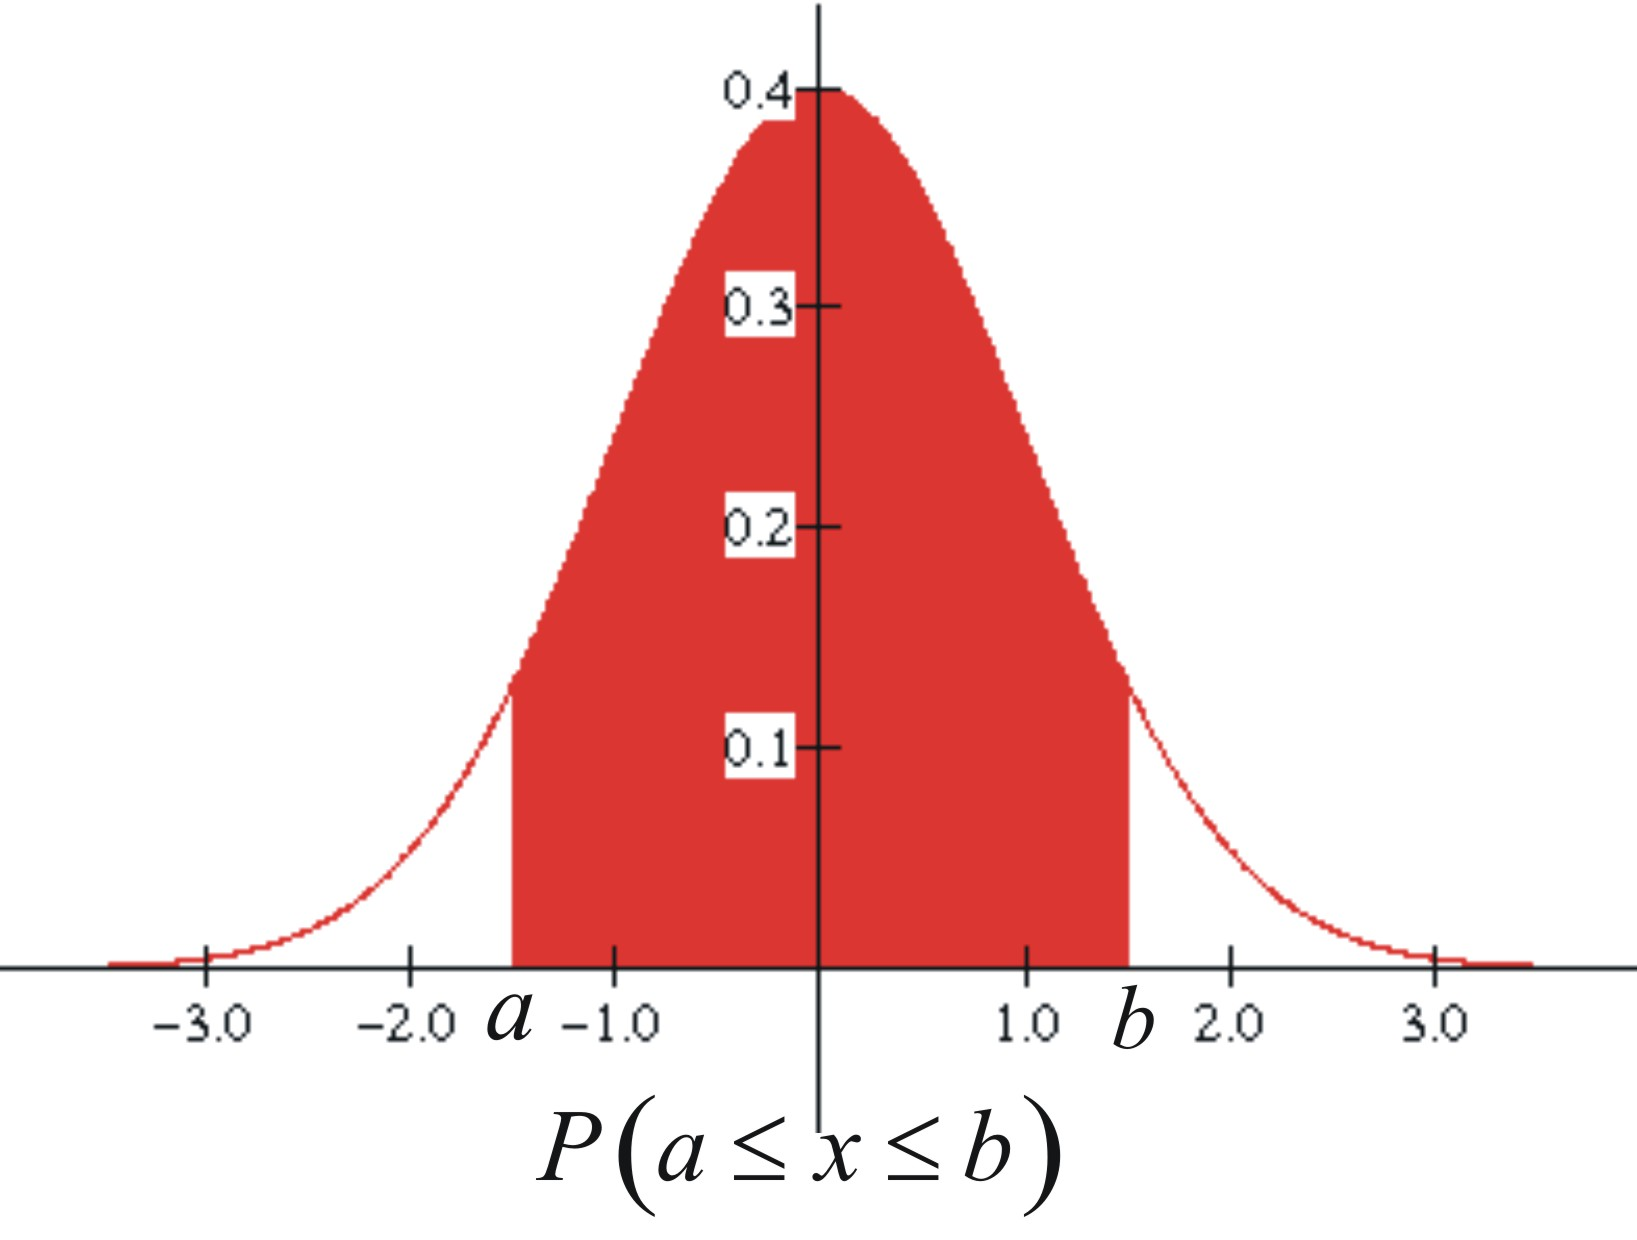
\includegraphics[width=7cm]{img813.jpg}
\label{fig4.5}
\end{center}

%EndExpansion


\begin{remark}
Al observar la gr�fica vemos que $P\left(  a\leq x\leq b\right) $
es el \'{a}rea bajo la curva de $f$
\end{remark}

\begin{remark}
Por ser $f$ integrable entonces la la probabilidad en un punto es nula, es
decir
\[
P\left(  X=a\right)  =P\left(  a\leq x\leq a\right)  =\int_{a}^{a}f\left(
x\right)  dx=0
\]

\end{remark}

\begin{remark}
Debido a lo anterior se tiene que

\begin{itemize}
\item La funci\'{o}n de densidad no es \'{u}nica

\item $P\left(  a\leq x\leq b\right)  =P\left(  a<x<b\right)  $

\item $P\left(  a\leq x\leq b\right)  =P\left(  a\leq x<b\right)  =P\left(
a<x\leq b\right)  $
\end{itemize}
\end{remark}

La funci\'{o}n de distribuci\'{o}n de una variable aleatoria, $F,$ continua se
define de modo que dado $x\epsilon$ $\rz$, $F\left(  x\right)  $ es la
probabilidad de que $X$ sea mayor o igual que $x,$ es decir
\[
\begin{array}
[c]{ccc}%
F:\rz & \longrightarrow & [0,1]\\
x & \longmapsto & F\left(  x\right)  =P\left(  x\geq X\right)  =\int_{-\infty
}^{x}f\left(  t\right)  dt
\end{array}
\]




\begin{proposition}
Dado un intervalo de la forma $(a,b]$, tenemos
\begin{align*}
P\left(  X\in(a,b]\right)   &  =\int_{a}^{b}f\left(  x\right)  dx\\
&  =\int_{-\infty}^{b}f\left(  x\right)  dx-\int_{-\infty}^{a}f\left(
x\right)  dx\\
&  =F\left(  b\right)  -F\left(  a\right)
\end{align*}
Se puede observar que la cantidad $F\left(  b\right)  -F\left(  a\right)  $
representa la masa de probabilidad extendida alo largo del intervalo $(a,b]$ .
Si dividimos esta cantidad por la longitud del intervalo,
\[
\frac{F\left(  b\right)  -F\left(  a\right)  }{b-a}
\]
tenemos la masa media de probabilidad por unidad de longitud en $(a,b]$, es
decir, su densidad media de probabilidad, ahora si
\[
\lim_{a\longrightarrow b}\frac{F\left(  b\right)  -F\left(  a\right)  }%
{b-a}=F^{\prime}\left(  b\right)  =f\left(  b\right)
\]
que es la densidad de probabilidad en el punto $b$
\end{proposition}

\begin{remark}
\begin{itemize}
\item Si $X$ es una variable continua la funci\'{o}n de distribuci\'{o}n $F$
es no decreciente, es decir si
\[
x_{1}<x_{2}\Longrightarrow F\left(  x_{2}\right)  \geq F\left(  x_{1}\right)
\]


\item esta funci\'{o}n es absolutamente convergente y se verifica
\begin{align*}
F\left(  -\infty\right)   &  =\lim_{x\longrightarrow-\infty}F\left(  x\right)
=0\\
F\left(  +\infty\right)   &  =\lim_{x\longrightarrow+\infty}F\left(  x\right)
\left(  1\right)
\end{align*}

\end{itemize}
\end{remark}

\begin{definition}
Funciones de probabilidad bivariada

\begin{enumerate}
\item Caso discreto: para cada resultado $\left(  x_{1i},x_{2j}\right)  $ de
$\left(  X_{1},X_{2}\right)  ,$ asociamos un n\'{u}mero
\[
f\left(  x_{1i},x_{2j}\right)  =P\left(  X_{1}=x_{1i},X_{2}=x_{2j}\right)
\]
donde
\begin{align*}
f\left(  x_{1i},x_{2j}\right)   &  \geq0\text{ }\\
\text{para todo }i  &  \in I,j\in J\text{ siendo }I,J\text{ conjuntos de
sub\'{\i}ndices}%
\end{align*}
y
\[
\sum_{i\in I}\sum_{j\in J}f\left(  x_{1i},x_{2j}\right)  =1
\]
Los valores $\left(  \left(  x_{1i},x_{2j}\right)  ,f\left(  x_{1i}%
,x_{2j}\right)  \right)  $ para todo $i\in I$ y $j\in J$ forman la
distribuci\'{o}n de probabilidad de $\left(  X_{1},X_{2}\right)  $

\item Caso continuo . Si $\left(  X_{1},X_{2}\right)  $ es un vector aleatorio
continuo con espacio del rango, $R,$ en $\rz^{2}$, entonces $f$, la
funci\'{o}n de densidad conjunta, tiene las siguientes propiedades
\[
f\left(  x_{1},x_{2}\right)  \geq0\text{ }\forall\left(  x_{1},x_{2}\right)
\in R
\]
y
\[
\int\int_{R}f\left(  x_{1},x_{2}\right)  dx_{1}dx_{2}=1
\]

\end{enumerate}
\end{definition}

\begin{definition}
Se dice que $\ n$ variables aleatorias \newline$X_{1},X_{2},X_{3},\cdots
,X_{k},$tiene una distribuci\'{o}n discreta conjunta si el vector
aleatorio\newline$X=\left(  X_{1},X_{2},X_{3},\cdots,X_{k}\right)  $ puede
tomar solamente un n\'{u}mero finito o una sucesi\'{o}n finita de valores
distintos posibles$\left(  x_{1},x_{2},x_{3},\cdots,x_{k}\right)  $ en
$\rz^{k}$. La funci\'{o}n de probabilidad cunjunta \ de $X_{1},X_{2}%
,X_{3},\cdots,X_{k}$ se define entonces como la funci\'{o}n $f$ tal que para
cualquier punto $x=\left(  x_{1},x_{2},x_{3},\cdots,x_{k}\right)  \in
A\subset$\rz$^{k},$%
\[
f\left(  x\right)  =P\left(  X=x\right)  \quad\forall x\in A
\]
donde $A$ es cualquier subconjunto de $\rz^{k}$
\[
P\left(  x\in A\right)  =\sum_{x\in A}f\left(  x\right)
\]

\end{definition}

\begin{definition}
Distribuciones continuas. se dice que n varibles aleatorias $X_{1},X_{2}%
,X_{3},\cdots,X_{k}$ tienen una distribuci\'{o}n conjunta continua si existe
una funci\'{o}n no negativa f definida sobre $\rz^{k}$ tal que para cualquier
subconjunto $A\subset\rz^{k}$
\begin{align*}
&  P\left(  \left(  X_{1},X_{2},X_{3},\cdots,X_{k}\right)  \in A\right) \\
&  =\int\cdots\int_{A}f\left(  x_{1},x_{2},x_{3},\cdots,x_{k}\right)
dx_{1}dx_{2}\cdots dx_{k}%
\end{align*}

\end{definition}

\begin{definition}
La f.d conjunta de k variables aleatorias\newline$X_{1},X_{2},X_{3}%
,\cdots,X_{k},$ se define como la funci\'{o}n $F$ cuyo valor en cualquier
punto $\left(  x_{1},x_{2},x_{3},\cdots,x_{k}\right)  $ de un espacio
k-dimensional
%TCIMACRO{\TeXButton{rz}{\rz}}%
%BeginExpansion
\rz
%EndExpansion
$^{k}$ est\'{a} dado por la relaci\'{o}n
\[
F\left(  x_{1},x_{2},x_{3},\cdots,x_{k}\right)  =P\left(  X_{1}\leq
x_{1},\cdots X_{k}\leq x_{k}\right)
\]

\end{definition}

\begin{remark}
\'{E}sta f.d satisface todas las propiedades de la f.d univariada.
\end{remark}

En el caso bivariado. Si $X$ y $Y$ son variables aleatorias con f.d.p conjunta
$f$ se tiene que
\[
F\left(  x,y\right)  =\int_{-\infty}^{x}\int_{-\infty}^{y}f\left(  u,v\right)
dudv
\]


Si la disribuci\'{o}n conjunta de $X_{1},X_{2},X_{3},\cdots,X_{k}$ es
continua, entonces la f.d.p conjunta f se puede obtener a partir de la f.d
conjunta F utilizando la relaci\'{o}n
\[
f\left(  x_{1},x_{2},x_{3},\cdots,x_{k}\right)  =\frac{\partial^{k}F\left(
x_{1},x_{2},x_{3},\cdots,x_{k}\right)  }{\partial x_{1}\partial x_{2}%
\cdots\partial x_{k}}
\]
para todos los puntos $\left(  x_{1},x_{2},x_{3},\cdots,x_{k}\right)  $ donde
exista la derivada.

En el caso bivariado
\[
f\left(  x,y\right)  =\frac{\partial^{2}F\left(  x,y\right)  }{\partial
x\partial y}
\]
$\forall\left(  x,y\right)  $ donde exista la derivada parcial de 2%
%TCIMACRO{\U{ba} }%
%BeginExpansion
${{}^o}$
%EndExpansion
orden

\begin{example}
Sup\'{o}ngase que la variable aleatoria X puede tomar solamente los valores
1,2,3, y que la variable Y puede tomar solamente los valores 1,2,3,4, donde la
f.p conjunta de X e Y es como indica la tabla\newline%
\begin{tabular}
[c]{|c|c|c|c|c|}\hline
$X|Y$ & 1 & 2 & 3 & 4\\\hline
1 & 0.1 & 0 & 0.1 & 0\\\hline
2 & 0.3 & 0 & 0.1 & 0.2\\\hline
3 & 0 & 0.2 & 0 & 0\\\hline
\end{tabular}
\newline determine los valores de $P\left(  X\geq2,Y\geq2\right)  $ y
$P\left(  X=1\right)  $

\begin{solution}
Sumando$f\left(  x.y\right)  $ sobre todos los valores de $x\geq2$ y de
$y\geq2,$ se obtiene
\begin{align*}
p\left(  X\geq2,Y\geq2\right)   &  =f\left(  2,2\right)  +f\left(  2,3\right)
+f\left(  2,4\right)  +\\
&  +f\left(  3,2\right)  +f\left(  3,3\right)  +f\left(  3,4\right) \\
&  =0.5\\
P\left(  X=1\right)   &  =\sum_{y=1}^{4}f\left(  1,y\right)  =0.2
\end{align*}

\end{solution}
\end{example}

\begin{center}

\end{center}

\begin{example}
Sup\'{o}ngase que la f.d.p conjunta de x e Y es la sigui\-ente
\[
f\left(  x,y\right)  =\left\{
\begin{array}
[c]{ccc}%
cx^{2}y & para & x^{2}\leq y\leq1\\
0 &  & \text{en otro caso}%
\end{array}
\right.
\]


\begin{itemize}
\item Determine el valor de la constante c

\item $P\left(  X\geq Y\right)  $
\end{itemize}

\begin{solution}
Sea el conjunto S de puntos $\left(  x,y\right)  $ para los que f$\left(
x,y\right)  >0$ est\'{a} representado en la figura 4.8 . puesto que $f\left(
x,y\right)  =0$ fuera de S, resulta que
\[
\int\int_{s}f\left(  x,y\right)  dxdy=\int_{-1}^{1}\int_{x^{2}}^{1}%
cx^{2}ydydx=\frac{4}{21}c
\]
y como esta integral debe ser 1, entonces c=$\frac{21}{4}$\newline$%
%TCIMACRO{\FRAME{itbpFU}{2.9706in}{1.9969in}{0in}{\Qcb{fig(a) Ejemplo 4.8}%
%}{\Qlb{fig 4.8a}}{imagen4.wmf}{\special{ language "Scientific Word";
%type "GRAPHIC";  maintain-aspect-ratio TRUE;  display "USEDEF";
%valid_file "F";  width 2.9706in;  height 1.9969in;  depth 0in;
%original-width 2.9274in;  original-height 1.9579in;  cropleft "0";
%croptop "1";  cropright "1";  cropbottom "0";
%filename '../Tacho/imagen4.wmf';file-properties "XNPEU";}}}%
%BeginExpansion
{\parbox[b]{2.9706in}{\begin{center}
\includegraphics[
natheight=1.957900in,
natwidth=2.927400in,
height=1.9969in,
width=2.9706in
]%
{imagen4.png}%
\\
fig(a) Ejemplo 4.8
\end{center}}}%
%EndExpansion
$

\begin{itemize}
\item Sea S$_{0}$ el conjunto donde x$\geq y$, entonces
\begin{align*}
\int\int_{S_{0}}f\left(  x,y\right)  dxdy &  =\\
\int_{0}^{1}\int_{x^{2}}^{x}\frac{21}{4}x^{2}ydydx &  =\frac{3}{20}%
\end{align*}%
%TCIMACRO{\FRAME{dhFU}{2.9706in}{1.9969in}{0pt}{\Qcb{Fig(b) Ejemplo 4.8}%
%}{\Qlb{fig 4.8b}}{imagen47.wmf}{\special{ language "Scientific Word";
%type "GRAPHIC";  maintain-aspect-ratio TRUE;  display "USEDEF";
%valid_file "F";  width 2.9706in;  height 1.9969in;  depth 0pt;
%original-width 2.9274in;  original-height 1.9579in;  cropleft "0";
%croptop "1";  cropright "1";  cropbottom "0";
%filename '../Tacho/Imagen47.wmf';file-properties "XNPEU";}}}%
%BeginExpansion
\begin{center}
\includegraphics[width=7cm]{imagen47.jpg}
\end{center}

%EndExpansion

\end{itemize}
\end{solution}
\end{example}

\begin{itemize}
\item En el caso discreto\ la distribuci\'{o}n marginal para $X_{1}$ y $X_{2}$
es
\begin{align*}
f\left(  x_{1}\right)   &  =\sum_{todo\,j}f\left(  x_{1i},x_{2j}\right)
\,\forall i=1,2,\cdots\\
f\left(  x_{2}\right)   &  =\sum_{todo\,i}f\left(  x_{1i},x_{2j}\right)
\,\forall j=1,2,\cdots
\end{align*}


\item En el caso continuo la distribuci\'{o}n marginal para $X_{1}$ y $X_{2}$
es
\begin{align*}
f\left(  x_{1}\right)   &  =\int_{-\infty}^{\infty}f\left(  x_{1}%
,x_{2}\right)  dx_{2}\\
f\left(  x_{2}\right)   &  =\int_{-\infty}^{\infty}f\left(  x_{1}%
,x_{2}\right)  dx_{1}%
\end{align*}

\end{itemize}
}% end fnz
}%
\item
\overlay{1}{%
compare to the result of the same slide with non-cumulative overlays
using:\newline
\Blue{\tt\fnz
\% switch-off cumulative overlays \newline
$\backslash$makeatletter
$\backslash$def$\backslash$pst@initoverlay\#1\{\%\newline
$\backslash$pst@Verb\{\%
$\backslash$tx@InitOL /TheOL (\#1) def\}\}\newline
$\backslash$makeatother
}\\%
\Red{
which doesn't really make sense here, but is needed in various situations
whenever you want to {\em replace objects} instead of {\em adding objects}}
}%
\end{dinglist}


\vspace*{-3mm}
\overlay{0}{%
\rule{50mm}{1pt}\\[-1ex]
{\fnz
$^\Red{*}$following the recipe outlined by Denis Girou in the seminar FAQ
(idea first suggested by Tomer KOL)\\[-1.6ex]
http://www.tug.org/applications/Seminar/Seminar-FAQ.html}
}%

\end{center}
\end{slide}
%%%%%%%%%%%

% switch-off cumulative overlays
\makeatletter
\def\pst@initoverlay#1{%
\pst@Verb{%
\tx@InitOL /TheOL (#1) def}}
\makeatother

%%%%%%%%%%%%% slide 3 %%%%%%%%%%%%%
\begin{slide}
\begin{center}

\psblurbox[fillstyle=solid,fillcolor=yellow,linecolor=red]
{\Blue{\huge\bf Title of this talk}}

\vspace{6mm}

we demonstrate different techniques for overlays:
\begin{dinglist}{253}
\overlay{1}{%
\Blue{\item\Black{
using the \DarkGreen{\tt $\backslash$overlay\{\#\}\{<stuff>\}} command for
cumulative overlays
}}% end color
}% end overlay
\overlay{2}{%
\DarkGreen{\item
\Black{
using the \DarkGreen{\tt $\backslash$overlay\{\#\}\{<stuff>\}} command
for non-cumulative overlays
}}% end color
}% end overlay
\overlay{3}{%
\Red{\item\Black{
repeating (almost) identical slides
}}% end color
}% end overlay
\end{dinglist}

\end{center}

\vspace*{20mm}
\rule{50mm}{1pt}\\[-1.6ex]
{\fnz
note: for the blurred shadow to the title box the file ``pst-blur.tex''
has to be included by \\[-1.6ex]
\DarkGreen{\tt $\backslash$usepackage\{pst-blur\}}}

\end{slide}
%%%%%%%%%%%

% switch-on cumulative overlays
\makeatletter
\def\pst@initoverlay#1{%
\pst@Verb{%
/BeginOL {dup (all) eq exch TheOL le or {IfVisible not {Visible
/IfVisible true def} if} {IfVisible {Invisible /IfVisible false def} if}
ifelse} def
\tx@InitOL /TheOL (#1) def}}
\makeatother

%%%%%%%%%%%%% slide 4 %%%%%%%%%%%%%
\begin{slide}
\begin{center}
\rput{0}(-2,3.4){%
one more example about cumulative overlays}
\rput{0}(0,0){%
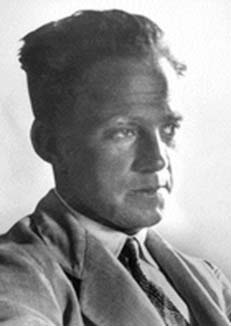
\includegraphics[width=.5\textwidth]{heisenberg.eps}}%
\overlay{1}{
\rput(2.59,2){
  \psframebox[fillstyle=solid,fillcolor=LightGray,linecolor=LightGray]
             {\DarkBlue{\LARGE$\geq \hbar/2$}}} }%
\rput{0}(2,-3.4){%
\ldots and the usefulness of patches \Red{\huge\Smiley}}

\end{center}
\end{slide}
%%%%%%%%%%%

% switch-off cumulative overlays
\makeatletter
\def\pst@initoverlay#1{%
\pst@Verb{%
\tx@InitOL /TheOL (#1) def}}
\makeatother

%%%%%%%%%% slide 5 %%% ??? %%%%%%%%%%%%%%%%%%%%%%%%%%%%%%%
\begin{slide}
\begin{center}

now we will display three examples\\
demonstrating nice ``overlay'' effects\\
by merely copying (almost) identical slides

\end{center}
\end{slide}
%%%%%%%%%%%

%%%%%%%%%%%%% slide 6 %%%%%%%%%%%%%
\begin{slide}

\Blue{\tt\fnz
$\backslash$begin\{slide\}
\newline
$\backslash$begin\{center\}
\newline
\qquad
$\backslash$rput(0,0)\{$\backslash$includegraphics[width=$\backslash$textwidth]\{transdist-Xi0.1.eps\}\}
\newline
$\backslash$end\{center\}$\backslash$end\{slide\}
\newline

\ldots\\
\ldots\\
\ldots\\
\ldots\\

$\backslash$begin\{slide\}
\newline
$\backslash$begin\{center\}
\newline
\qquad
$\backslash$rput(0,0)\{$\backslash$includegraphics[width=$\backslash$textwidth]\{transdist-Xi0.6.eps\}\}
\newline
$\backslash$end\{center\}
\newline
$\backslash$end\{slide\}
\newline
}% end \fnz


\end{slide}
%%%%%%%%%%%

\renewcommand{\headtext}{geometrical interpretation of GPDs}

%%%%%%%%%%%%% slide 7 %%%%%%%%%%%%%
\begin{slide}
\begin{center}
\rput{0}(0,0){%
\includegraphics[width=\textwidth]{transdist-Xi0.0.eps}}%
\end{center}
\end{slide}
%%%%%%%%%%%

%%%%%%%%%%%%% slide 8 %%%%%%%%%%%%%
\begin{slide}
\begin{center}
\rput{0}(0,0){%
\includegraphics[width=\textwidth]{transdist-Xi0.1.eps}}%
\end{center}
\end{slide}
%%%%%%%%%%%

%%%%%%%%%%%%% slide 9 %%%%%%%%%%%%%
\begin{slide}
\begin{center}
\rput{0}(0,0){%
\includegraphics[width=\textwidth]{transdist-Xi0.2.eps}}%
\end{center}
\end{slide}
%%%%%%%%%%%

%%%%%%%%%%%%% slide 10 %%%%%%%%%%%%
\begin{slide}
\begin{center}
\rput{0}(0,0){%
\includegraphics[width=\textwidth]{transdist-Xi0.3.eps}}%
\end{center}
\end{slide}
%%%%%%%%%%%

%%%%%%%%%%%%% slide 11 %%%%%%%%%%%%%
\begin{slide}
\begin{center}
\rput{0}(0,0){%
\includegraphics[width=\textwidth]{transdist-Xi0.4.eps}}%
\end{center}
\end{slide}
%%%%%%%%%%%

%%%%%%%%%%%%% slide 12 %%%%%%%%%%%%%
\begin{slide}
\begin{center}
\rput{0}(0,0){%
\includegraphics[width=\textwidth]{transdist-Xi0.5.eps}}%
\end{center}
\end{slide}
%%%%%%%%%%%

%%%%%%%%%%%%% slide 13 %%%%%%%%%%%%%
\begin{slide}
\begin{center}
\rput{0}(0,0){%
\includegraphics[width=\textwidth]{transdist-Xi0.6.eps}}%
\end{center}
\end{slide}
%%%%%%%%%%%

\renewcommand{\headtext}{exclusive reactions}

%%%%%%%%%% slide 14%%% ??? %%%%%%%%%%%%%%%%%%%%%%%%%%%%%%%
\begin{slide}
\begin{center}

\font\bighelv=phvb at .7cm
\rput{0}(0,0){%
\psshadow{\bighelv \LightBlue{advantages of being exclusive \ldots}}
}%
\rput{0}(0,0){%
         {\bighelv \Blue{advantages of being exclusive \ldots}}
}%

\font\midhelv=phvb at .4cm
\rput{0}(2,-1){%
\psshadow{\midhelv \LightRed{sensitivity to reaction mechanisms}}
}%
\rput{0}(2,-1){%
         {\midhelv \Red{sensitivity to reaction mechanisms}}
}%

\font\bighelv=phvb at .6cm
\rput{0}(2,-2){%
\psshadow{\bighelv \LightRed{generalised parton distributions}}
}%
\rput{0}(2,-2){%
         {\bighelv \Red{generalised parton distributions}}
}%

\end{center}
\end{slide}
%%%%%%%%%%%%

%%%%%%%%%% slide 15 %% ??? %%%%%%%%%%%%%%%%%%%%%%%%%%%%%%%
\begin{slide}
\begin{center}

\font\bighelv=phvb at .7cm
\rput{0}(0,0){%
\psshadow{\bighelv \VeryLightBlue{advantages of being exclusive \ldots}}
}%
\rput{0}(0,0){%
         {\bighelv \LightBlue{advantages of being exclusive \ldots}}
}%

\font\midhelv=phvb at .4cm
\rput{0}(2,-1){%
\psshadow{\midhelv \LightRed{sensitivity to reaction mechanisms}}
}%
\rput{0}(2,-1){%
         {\midhelv \Red{sensitivity to reaction mechanisms}}
}%

\font\bighelv=phvb at .6cm
\rput{0}(2,-2){%
\psshadow{\bighelv \VeryLightRed{generalised parton distributions}}
}%
\rput{0}(2,-2){%
         {\bighelv \LightRed{generalised parton distributions}}
}%

\end{center}
\end{slide}
%%%%%%%%%%%%

%%%%%%%%%% slide ? %%% ??? %%%%%%%%%%%%%%%%%%%%%%%%%%%%%%%
\begin{slide}
\begin{center}

\font\bighelv=phvb at .7cm
\rput{0}(0,0){%
\psshadow{\bighelv \VeryLightBlue{advantages of being exclusive \ldots}}
}%
\rput{0}(0,0){%
         {\bighelv \LightBlue{advantages of being exclusive \ldots}}
}%

\font\midhelv=phvb at .4cm
\rput{0}(2,-1){%
\psshadow{\midhelv \VeryLightRed{sensitivity to reaction mechanisms}}
}%
\rput{0}(2,-1){%
         {\midhelv \LightRed{sensitivity to reaction mechanisms}}
}%

\font\bighelv=phvb at .6cm
\rput{0}(2,-2){%
\psshadow{\bighelv \LightRed{generalised parton distributions}}
}%
\rput{0}(2,-2){%
         {\bighelv \Red{generalised parton distributions}}
}%

\end{center}
\end{slide}
%%%%%%%%%%%%

%%%%%%%%%% slide ?a %%% GPD table %%%%%%%%%%%%%%%%%%%%%%%%%%%%%%%
\begin{slide}
\begin{center}

\rput{0}(4.4,-0.5){\psblurbox[fillstyle=solid,fillcolor=LightBlue]
{\Red{`GPDs link many different quantities'}}}

\psset{unit=1.4truemm}
\psset{arrowinset=0,linewidth=1pt}

%\sffamily
\renewcommand{\baselinestretch}{0.7}

\begin{pspicture}(165,120)
%
% SPDs
\rput{0}(85,60){\rnode{spd}{\psovalbox[linecolor=Blue,linewidth=2pt,
fillstyle=solid,fillcolor=LightBlue,shadow=true,blur=true,framesep=5truemm]
{\large\Blue{\bf GPDs}}}}
%
% orbital angular momentum
\rput{0}(150,60){\rnode{ang}{\psframebox[linecolor=Yellow,fillstyle=solid,
fillcolor=LightBlue,framesep=3truemm,framearc=.3]
%{\Large $J_q$, $J_G$}}}
{\small \begin{tabular}{c} orbital angular\\ momentum\\[2mm]
transverse localisation\end{tabular}}}}
\ncline[nodesep=2truemm,linewidth=2pt,linecolor=Blue,
linestyle=dashed,dash=1.5pt 1.5pt]
{->}{spd}{ang}
%
% FF
\rput{0}(115,100){\rnode{ff}{\psframebox[linecolor=Red,
fillstyle=solid,fillcolor=LightYellow,
shadow=true,blur=true,
shadowcolor=Red,shadowsize=2pt,blurradius=1pt,
framesep=2truemm,framearc=.3]
{\fnz \begin{tabular}{c} form\\ factors \end{tabular}}}}
\ncline[nodesep=2truemm,linewidth=2pt,linestyle=dashed,dash=1.5pt 1.5pt]
{<->}{spd}{ff}
%\ncarc[nodesep=3truemm]{->}{spd}{ff}
%\ncarc[nodesep=3truemm]{->}{ff}{spd}
%
% WACS
\rput{0}(75,100){\rnode{wacs}{\psframebox[linecolor=Red,
fillstyle=solid,fillcolor=LightYellow,
shadow=true,blur=true,
shadowcolor=Red,shadowsize=2pt,blurradius=1pt,
framesep=2truemm,framearc=.3]
{\fnz \begin{tabular}{c} wide angle\\ Compton\\ scattering\end{tabular}}}}
\ncline[nodesep=2truemm,linewidth=2pt,linestyle=dashed,dash=1.5pt 1.5pt]
{<->}{spd}{wacs}
%
% DIS
\rput{0}(115,20){\rnode{dis}{\psframebox[linecolor=Red,
fillstyle=solid,fillcolor=LightYellow,
shadow=true,blur=true,
shadowcolor=Red,shadowsize=2pt,blurradius=1pt,
framesep=2truemm,framearc=.3]
{\fnz {
\begin{tabular}{c} deep inelastic\\ scattering\\PDFs \end{tabular}}}}}
\ncline[nodesep=2truemm,linewidth=2pt,linestyle=dashed,dash=1.5pt 1.5pt]
{<->}{spd}{dis}
%
% Meson production
\rput{0}(70,20){\rnode{mes}{\psframebox[linecolor=Red,
fillstyle=solid,fillcolor=LightYellow,
shadow=true,blur=true,
shadowcolor=Red,shadowsize=2pt,blurradius=1pt,
framesep=2truemm,framearc=.3]
{\fnz \begin{tabular}{c} exclusive\\ meson production\\
{deep virtual/}large $t$ \end{tabular}}}}
\ncline[nodesep=2truemm,linewidth=2pt,linestyle=dashed,dash=1.5pt 1.5pt]
{<->}{spd}{mes}
%
% DVCS
\rput{0}(25,95){\rnode{dvcs}{\psframebox[linecolor=Red,
fillstyle=solid,fillcolor=LightYellow,
shadow=true,blur=true,
shadowcolor=Red,shadowsize=2pt,blurradius=1pt,
framesep=2truemm,framearc=.3]
{\fnz {
\begin{tabular}{c} deeply virtual\\ Compton\\
scattering \end{tabular}}}}}
\ncline[nodesep=2truemm,linewidth=2pt,linestyle=dashed,dash=1.5pt 1.5pt]
{<->}{spd}{dvcs}
%
% TCS
\rput{0}(15,65){\rnode{tcs}{\psframebox[linecolor=Red,
fillstyle=solid,fillcolor=LightYellow,
shadow=true,blur=true,
shadowcolor=Red,shadowsize=2pt,blurradius=1pt,
framesep=2truemm,framearc=.3]
{\fnz {
\begin{tabular}{c} timelike\\ Compton\\
scattering \end{tabular}}}}}
\ncline[nodesep=2truemm,linewidth=2pt,linestyle=dashed,dash=1.5pt 1.5pt]
{<->}{spd}{tcs}
%
% pp/pipi
\rput{0}(15,35){\rnode{ppbar}{\psframebox[linecolor=Red,
fillstyle=solid,fillcolor=LightYellow,
shadow=true,blur=true,
shadowcolor=Red,shadowsize=2pt,blurradius=1pt,
framesep=2truemm,framearc=.3]
{\fnz {
\begin{tabular}{c}
$p\bar p$ annihilation\\[1mm]
\hline\\
$\gamma\gamma\to\pi\pi$, $\gamma\gamma\to KK$
\end{tabular}}}}}
\ncline[nodesep=2truemm,linewidth=2pt,linestyle=dashed,dash=1.5pt 1.5pt,
linecolor=gray]
{<->}{spd}{ppbar}
%
\end{pspicture}

\end{center}
\end{slide}
%%%%%%%%%%%%

%%%%%%%%%% slide ?b %%% GPD table %%%%%%%%%%%%%%%%%%%%%%%%%%%%%%%
\begin{slide}
\begin{center}

\rput{0}(4.4,-0.5){\psblurbox[fillstyle=solid,fillcolor=LightBlue]
{\Red{`GPDs link many different quantities'}}}

\psset{unit=1.4truemm}
\psset{arrowinset=0,linewidth=1pt}

%\sffamily
\renewcommand{\baselinestretch}{0.7}

\begin{pspicture}(165,120)
%
% SPDs
\rput{0}(85,60){\rnode{spd}{\psovalbox[linecolor=Blue,linewidth=2pt,
fillstyle=solid,fillcolor=LightBlue,shadow=true,blur=true,framesep=5truemm]
{\large\Blue{\bf GPDs}}}}
%
% orbital angular momentum
\rput{0}(150,60){\rnode{ang}{\psframebox[linecolor=Yellow,fillstyle=solid,
fillcolor=LightBlue,framesep=3truemm,framearc=.3]
%{\Large $J_q$, $J_G$}}}
{\small \begin{tabular}{c} orbital angular\\ momentum\\[2mm]
transverse localisation\end{tabular}}}}
\ncline[nodesep=2truemm,linewidth=2pt,linecolor=Blue,
linestyle=dashed,dash=1.5pt 1.5pt]
{->}{spd}{ang}
%
% FF
\rput{0}(115,100){\rnode{ff}{\psframebox[linecolor=Red,
fillstyle=solid,fillcolor=LightYellow,
shadow=true,blur=true,
shadowcolor=Red,shadowsize=12pt,blurradius=6pt,
framesep=2truemm,framearc=.3]
{\fnz \begin{tabular}{c} form\\ factors \end{tabular}}}}
\ncline[nodesep=2truemm,linewidth=2pt,linestyle=dashed,dash=1.5pt 1.5pt]
{<->}{spd}{ff}
%\ncarc[nodesep=3truemm]{->}{spd}{ff}
%\ncarc[nodesep=3truemm]{->}{ff}{spd}
%
% WACS
\rput{0}(75,100){\rnode{wacs}{\psframebox[linecolor=Red,
fillstyle=solid,fillcolor=LightYellow,
shadow=true,blur=true,
shadowcolor=Red,shadowsize=12pt,blurradius=6pt,
framesep=2truemm,framearc=.3]
{\fnz \begin{tabular}{c} wide angle\\ Compton\\ scattering\end{tabular}}}}
\ncline[nodesep=2truemm,linewidth=2pt,linestyle=dashed,dash=1.5pt 1.5pt]
{<->}{spd}{wacs}
%
% DIS
\rput{0}(115,20){\rnode{dis}{\psframebox[linecolor=LightRed,
fillstyle=solid,fillcolor=VeryLightYellow,
shadow=true,blur=true,
shadowcolor=Red,shadowsize=2pt,blurradius=1pt,
framesep=2truemm,framearc=.3]
{\fnz \Gray{
\begin{tabular}{c} deep inelastic\\ scattering\\PDFs \end{tabular}}}}}
\ncline[nodesep=2truemm,linewidth=2pt,linestyle=dashed,dash=1.5pt 1.5pt]
{<->}{spd}{dis}
%
% Meson production
\rput{0}(70,20){\rnode{mes}{\psframebox[linecolor=Red,
fillstyle=solid,fillcolor=LightYellow,
shadow=true,blur=true,
shadowcolor=Red,shadowsize=12pt,blurradius=6pt,
framesep=2truemm,framearc=.3]
{\fnz \begin{tabular}{c} exclusive\\ meson production\\
\Gray{deep virtual/}large $t$ \end{tabular}}}}
\ncline[nodesep=2truemm,linewidth=2pt,linestyle=dashed,dash=1.5pt 1.5pt]
{<->}{spd}{mes}
%
% DVCS
\rput{0}(25,95){\rnode{dvcs}{\psframebox[linecolor=LightRed,
fillstyle=solid,fillcolor=VeryLightYellow,
shadow=true,blur=true,
shadowcolor=Red,shadowsize=2pt,blurradius=1pt,
framesep=2truemm,framearc=.3]
{\fnz \Gray{
\begin{tabular}{c} deeply virtual\\ Compton\\
scattering \end{tabular}}}}}
\ncline[nodesep=2truemm,linewidth=2pt,linestyle=dashed,dash=1.5pt 1.5pt]
{<->}{spd}{dvcs}
%
% TCS
\rput{0}(15,65){\rnode{tcs}{\psframebox[linecolor=LightRed,
fillstyle=solid,fillcolor=VeryLightYellow,
shadow=true,blur=true,
shadowcolor=Red,shadowsize=2pt,blurradius=1pt,
framesep=2truemm,framearc=.3]
{\fnz \Gray{
\begin{tabular}{c} timelike\\ Compton\\
scattering \end{tabular}}}}}
\ncline[nodesep=2truemm,linewidth=2pt,linestyle=dashed,dash=1.5pt 1.5pt]
{<->}{spd}{tcs}
%
% pp/pipi
\rput{0}(15,35){\rnode{ppbar}{\psframebox[linecolor=Red,
fillstyle=solid,fillcolor=LightYellow,
shadow=true,blur=true,
shadowcolor=Red,shadowsize=12pt,blurradius=6pt,
framesep=2truemm,framearc=.3]
{\fnz {
\begin{tabular}{c}
$p\bar p$ annihilation\\[1mm]
\hline\\
$\gamma\gamma\to\pi\pi$, $\gamma\gamma\to KK$
\end{tabular}}}}}
\ncline[nodesep=2truemm,linewidth=2pt,linestyle=dashed,dash=1.5pt 1.5pt,
linecolor=gray]
{<->}{spd}{ppbar}
%
\end{pspicture}

\end{center}
\end{slide}
%%%%%%%%%%%%

%%%%%%%%%% slide ?c %%% GPD table %%%%%%%%%%%%%%%%%%%%%%%%%%%%%%%
\begin{slide}
\begin{center}

\rput{0}(4.4,-0.5){\psblurbox[fillstyle=solid,fillcolor=LightBlue]
{\Red{`GPDs link many different quantities'}}}

\psset{unit=1.4truemm}
\psset{arrowinset=0,linewidth=1pt}

%\sffamily
\renewcommand{\baselinestretch}{0.7}

\begin{pspicture}(165,120)
%
% SPDs
\rput{0}(85,60){\rnode{spd}{\psovalbox[linecolor=Blue,linewidth=2pt,
fillstyle=solid,fillcolor=LightBlue,shadow=true,blur=true,framesep=5truemm]
{\large\Blue{\bf GPDs}}}}
%
% orbital angular momentum
\rput{0}(150,60){\rnode{ang}{\psframebox[linecolor=Yellow,fillstyle=solid,
fillcolor=LightBlue,framesep=3truemm,framearc=.3]
%{\Large $J_q$, $J_G$}}}
{\small \begin{tabular}{c} orbital angular\\ momentum\\[2mm]
transverse localisation\end{tabular}}}}
\ncline[nodesep=2truemm,linewidth=2pt,linecolor=Blue,
linestyle=dashed,dash=1.5pt 1.5pt]
{->}{spd}{ang}
%
% FF
\rput{0}(115,100){\rnode{ff}{\psframebox[linecolor=Red,
fillstyle=solid,fillcolor=LightYellow,
shadow=true,blur=true,
shadowcolor=Red,shadowsize=12pt,blurradius=6pt,
framesep=2truemm,framearc=.3]
{\fnz \begin{tabular}{c} form\\ factors \end{tabular}}}}
\ncline[nodesep=2truemm,linewidth=2pt,linestyle=dashed,dash=1.5pt 1.5pt]
{<->}{spd}{ff}
%\ncarc[nodesep=3truemm]{->}{spd}{ff}
%\ncarc[nodesep=3truemm]{->}{ff}{spd}
%
% WACS
\rput{0}(75,100){\rnode{wacs}{\psframebox[linecolor=LightRed,
fillstyle=solid,fillcolor=VeryLightYellow,
shadow=true,blur=true,
shadowcolor=Red,shadowsize=2pt,blurradius=1pt,
framesep=2truemm,framearc=.3]
{\fnz \Gray{
\begin{tabular}{c} wide angle\\ Compton\\ scattering\end{tabular}}}}}
\ncline[nodesep=2truemm,linewidth=2pt,linestyle=dashed,dash=1.5pt 1.5pt]
{<->}{spd}{wacs}
%
% DIS
\rput{0}(115,20){\rnode{dis}{\psframebox[linecolor=Red,
fillstyle=solid,fillcolor=LightYellow,
shadow=true,blur=true,
shadowcolor=Red,shadowsize=12pt,blurradius=6pt,
framesep=2truemm,framearc=.3]
{\fnz {
\begin{tabular}{c} deep inelastic\\ scattering\\PDFs \end{tabular}}}}}
\ncline[nodesep=2truemm,linewidth=2pt,linestyle=dashed,dash=1.5pt 1.5pt]
{<->}{spd}{dis}
%
% Meson production
\rput{0}(70,20){\rnode{mes}{\psframebox[linecolor=Red,
fillstyle=solid,fillcolor=LightYellow,
shadow=true,blur=true,
shadowcolor=Red,shadowsize=12pt,blurradius=6pt,
framesep=2truemm,framearc=.3]
{\fnz \begin{tabular}{c} exclusive\\ meson production\\
{deep virtual}\Gray{/large $t$} \end{tabular}}}}
\ncline[nodesep=2truemm,linewidth=2pt,linestyle=dashed,dash=1.5pt 1.5pt]
{<->}{spd}{mes}
%
% DVCS
\rput{0}(25,95){\rnode{dvcs}{\psframebox[linecolor=Red,
fillstyle=solid,fillcolor=LightYellow,
shadow=true,blur=true,
shadowcolor=Red,shadowsize=12pt,blurradius=6pt,
framesep=2truemm,framearc=.3]
{\fnz {
\begin{tabular}{c} deeply virtual\\ Compton\\
scattering \end{tabular}}}}}
\ncline[nodesep=2truemm,linewidth=2pt,linestyle=dashed,dash=1.5pt 1.5pt]
{<->}{spd}{dvcs}
%
% TCS
\rput{0}(15,65){\rnode{tcs}{\psframebox[linecolor=Red,
fillstyle=solid,fillcolor=LightYellow,
shadow=true,blur=true,
shadowcolor=Red,shadowsize=12pt,blurradius=6pt,
framesep=2truemm,framearc=.3]
{\fnz {
\begin{tabular}{c} timelike\\ Compton\\
scattering \end{tabular}}}}}
\ncline[nodesep=2truemm,linewidth=2pt,linestyle=dashed,dash=1.5pt 1.5pt]
{<->}{spd}{tcs}
%
% pp/pipi
\rput{0}(15,35){\rnode{ppbar}{\psframebox[linecolor=LightRed,
fillstyle=solid,fillcolor=VeryLightYellow,
shadow=true,blur=true,
shadowcolor=Red,shadowsize=2pt,blurradius=1pt,
framesep=2truemm,framearc=.3]
{\fnz \Gray{
\begin{tabular}{c}
$p\bar p$ annihilation\\[1mm]
\hline\\
$\gamma\gamma\to\pi\pi$, $\gamma\gamma\to KK$
\end{tabular}}}}}
\ncline[nodesep=2truemm,linewidth=2pt,linestyle=dashed,dash=1.5pt 1.5pt,
linecolor=gray]
{<->}{spd}{ppbar}
%
\end{pspicture}

\end{center}
\end{slide}
%%%%%%%%%%%%

\renewcommand{\headtext}{the end}

%%%%%%%%%%%%% slide ? %%%%%%%%%%%%%
\begin{slide}
\begin{center}

{\huge\bf the end}

and this is the last slide

\end{center}
\end{slide}

\end{document}
